\documentclass[3p,twocolumn]{elsarticle}

\usepackage{ctex}
\usepackage[T1]{fontenc}
\usepackage{textcomp}
\usepackage{lineno,hyperref}
\usepackage{amsmath,amssymb,amsfonts,amsthm}
\usepackage{graphicx}
\usepackage{booktabs}
\usepackage{multirow}
\usepackage{siunitx}
\usepackage{caption}
\usepackage{subcaption}
\usepackage{xcolor}
\usepackage{threeparttable}
\usepackage{array}
\usepackage{enumitem}
\usepackage[expansion=false]{microtype}
\usepackage{tabularx}
\usepackage{ragged2e}
\usepackage{url}

\journal{Applied Energy}
\bibliographystyle{elsarticle-num}

\hypersetup{
    colorlinks=true,
    linkcolor=blue,
    citecolor=blue,
    urlcolor=blue,
    pdfencoding=auto,
    psdextra
}
\pdfstringdefDisableCommands{\def\corref#1{}}

% 中文定理与命题环境定义
\newtheorem{theorem}{定理}
\newtheorem{proposition}{命题}
\newtheorem{lemma}{引理}
\newtheorem{corollary}{推论}
\theoremstyle{definition}
\newtheorem{definition}{定义}
\newtheorem{hypothesis}{假设}
\theoremstyle{remark}
\newtheorem{remark}{注记}
\newtheorem{example}{反例}

\usepackage{dblfloatfix}

% 浮动体排版优化
\renewcommand{\topfraction}{0.95}
\renewcommand{\bottomfraction}{0.95}
\renewcommand{\textfraction}{0.05}
\renewcommand{\floatpagefraction}{0.70}
\renewcommand{\dbltopfraction}{0.95}
\renewcommand{\dblfloatpagefraction}{0.70}
\setcounter{topnumber}{5}
\setcounter{bottomnumber}{5}
\setcounter{totalnumber}{10}
\setcounter{dbltopnumber}{5}

\graphicspath{{figures/}}

\begin{document}

\begin{frontmatter}

\title{风电预测中物理约束决策价值的实证审计}

\author[1]{李俊宇\corref{cor1}}
\ead{ljylikezmn999@gmail.com}

\author[1]{杜俊涛}

\address[1]{智能电力系统与计算能源交叉研究组，中国}

\cortext[cor1]{通信作者}

\begin{highlights}
\item 结合文献审计、代码核查与风场受控实验，检验风电物理约束预测的收益归因依据。
\item 46项被审计研究中44项缺失公开代码，50\%采用模块级消融混淆了先验贡献。
\item 代码核查识别出公开实现的散度参数方向与论文定义不符，改变了梯度尺度。
\item 强约束下打乱物理先验导致决策损失激增68.1\%，揭示出显著的先验误设脆弱性。
\item 退化零申报探针揭示了孤立未对冲平衡现金流无法单独衡量预测模型优劣。
\end{highlights}

\begin{abstract}
物理约束模型的预测误差下降，并不足以说明收益来自先验中的有效信息，也不能直接证明其决策价值。本文结合文献审计、代码核查与三座英国风场的受控实验，检验风电预测中约束收益的归因依据。在纳入的 46 项研究中，审计账本未记录运行负效应报告，44 项未找到公开代码，23 项通过移除网络模块进行消融，难以单独识别先验贡献。在同骨干、相同决策校准的比较中，历史功率曲线先验的效果随实验条件变化：Penmanshiel 上，强约束使归一化非对称决策损失平均下降 1.28\%，打乱风速—功率映射则使其上升 61.2\%。在另外两站，固定历史先验在较短模型训练窗口下带来较低的平均损失，窗口扩大后该优势消退。代码核查发现一项公开实现的散度参数方向与文中定义不符；零申报对照进一步表明，孤立的不平衡现金流无法单独衡量预测能力。这些结果支持对先验来源、实现语义和决策指标分别验证，并将约束收益限定在实际测试的先验与数据条件内。
\end{abstract}

\begin{keyword}
物理约束深度学习 \sep 风电功率预测 \sep 预测-决策脱钩 \sep 条件归纳偏置 \sep 系统性实证审计 \sep 软件实现保真度 \sep 机器学习可复现性
\end{keyword}

\end{frontmatter}

\section{引言与问题界定}
\label{sec:intro}

在电力系统运行与电力现货市场中，风电功率预测的实际运行价值根本上取决于日前发电计划申报与实时平衡调度中的非对称决策损失 \cite{holttinen2021,weron2014}。在典型的两部制平衡结算规则下，预测不足导致的电网短缺惩罚与多发导致的弃电回收价格存在显著差异。在这种非对称决策工况下，均方根误差 (RMSE) 或平均绝对误差 (MAE) 等传统对称回归指标无法代表下行经济风险与电网备用安全敞口 \cite{lipton2019}。为提升模型泛化性能并防止产生违背机组运行特性的反常预测，大量研究倡导将气动极限、经验功率曲线或运动学方程直接融入深度神经网络结构与损失函数中 \cite{raissi2019physics,karniadakis2021physics,sheng2025annreview,pct2026}。这一研究范式普遍建立在一个核心前提之上：所报告的预测误差下降，能够直接归因于物理约束中编码的有效领域知识。

然而，现行的文献报告惯例、开源代码赤字与消融实验设计掩盖了这一归因基础。首先，现有文献几乎普遍报告积极收益，极少探讨物理先验的失效工况或负面权衡。其次，公开可复现的源代码极其匮乏，导致算法的底层计算图执行往往缺乏独立检验 \cite{kapoor2023,pineau2021}。再次，现有消融实验普遍通过直接剔除多层神经网络子模块（如特征编码通道或注意力模块）来评估物理约束，而非在保持网络容量不变的前提下隔离物理惩罚权重 $\lambda$。这种粗粒度消融不可避免地将网络参数容量与物理归纳偏置混为一谈。因此，现有文献留下了一个核心追问：物理约束带来的收益，究竟来自有效的先验信息，还是其他因素？这些收益在什么条件下会消失或逆转？

为了从经验上检验物理约束收益的归因依据，我们在三座英国商业风电场（Kelmarsh、Hill of Towie 与 Penmanshiel）开展了受控实证审计。在保持预测网络骨干 (DLinear) 与验证集后验分位数偏移校准完全一致的前提下，我们引入形式与权重匹配的伪打乱先验作为阴性对照，系统扰动先验参数并改变模型训练窗口。受控实验表明，物理先验的效益高度依赖于具体数据条件与约束设置：
\begin{enumerate}[leftmargin=*]
\item \textbf{先验特异性与误设脆弱性}：在 Penmanshiel 样本受限工况下（$N_{\text{train}}=1{,}583$），施加强功率曲线先验使归一化非对称决策损失降低 1.22\%。然而，在保持损失形式、模型架构与正则化权重完全相同的条件下，打乱风速与功率的物理对应关系会导致决策损失激增 68.1\%。这一鲜明对比证实：虽然有效领域知识在数据匮乏时能提供可测量的归纳保护，但强正则化下模型对先验误设表现出极高的脆弱性。
\item \textbf{信息预算与样本机制}：在不同训练样本预算的评估中，固定历史经验先验在较短训练窗口下（如 $N=500$，约对应 21 天近期样本）展现出边际优势。然而，由于该经验先验是在全年完整历史数据（7 至 10 个月）上拟合所得，它实际为模型注入了显著的额外历史信息预算。随着模型自身训练样本扩大至 $N=5{,}000$，先验优势逐渐消退并发生轻微反转，刚性的历史曲线反而限制了模型适应局部动态变化的能力。
\item \textbf{实现偏离与市场指标脱钩}：在软件执行层面，对开源计算图的核查发现物理约束 Transformer (PCT) 的 Jensen--Shannon (JS) 散度损失函数存在反向参数传递，引发了非对称的反向梯度缩放。在下游市场评估中，对结算机制的数理分析表明，孤立的未对冲平衡现金流与预测能力存在结构性脱钩：退化零申报基准（$q \equiv 0$）无需任何预测能力即可机械获取巨额名义现金流。
\end{enumerate}

\subsection{主要研究贡献}
本文从文献报告规范、底层软件执行与不平衡结算及决策风险诊断三个相互支撑的维度，对物理约束风电预测展开系统实证审计：
\begin{itemize}[leftmargin=*]
\item \textbf{文献报告规范与代码可用性范围界定审计}：在 PRISMA-ScR 指导下，我们对 46 项当代代表性研究（2023--2026）展开全生命周期范围界定审计，量化了失效边界报告的缺失（0/46，0.0\%）、开源代码的严重赤字（44/46，95.7\%）以及模块级结构消融的普遍混淆（23/46，50.0\%）。
\item \textbf{骨干对齐的前瞻性受控消融基准}：通过在 10 卡专用物理 GPU 集群上跨三座风电场（各站 3--4 个独立随机种子）将真实先验与尺度对齐的伪打乱阴性对照进行成对消融，利用形式与权重对齐的阴性对照区分领域特定先验效应与非特异性数值平滑，刻画了物理约束收益在样本规模、先验扰动与气象代理时效错配下的实证边界。
\item \textbf{底层计算图核查与结算脱钩诊断}：我们揭示了开源物理约束软件中存在的实现偏离，并通过数理与实证分析阐明了为何孤立的单边平衡现金流不能作为预测质量的评价指标，确立了以归一化非对称调度损失为核心的决策理论审计框架。
\end{itemize}

\paragraph{研究范畴与方法边界}
本文确立四项明确的实证审计范畴：首先，文献范围界定审计刻画纳入的 46 项当代研究（38 篇期刊论文与 8 篇预印本，2023--2026）的报告与消融规范，反映该范围界定样本内的报道现状而非断言全领域通用属性；其次，软件审计基于开源 PCT 代码库（commit \texttt{65941ec}）分析其静态计算图实现保真度；第三，前瞻性受控消融实验在三座商业风电场上以对齐的 DLinear 为基准刻画边界行为，并辅以 PatchTST 作为结构敏感性探针；第四，下游市场评估基于英国平衡机制两部制非对称短缺清算规则开展不平衡结算与决策风险诊断，揭示评价指标的病态反常而非承诺全组合商业清算。上述四个维度共同构成扎实的实证证据链。

\section{相关工作与学术定位}
\label{sec:related_work}

为清晰确立本实证审计工作在能源信息学与应用机器学习交叉领域的学术坐标，我们系统梳理三个相交的研究脉络：(i) 物理约束预测中的先验知识注入范式；(ii) 风电预测的基准评测、鲁棒性与决策价值度量；以及 (iii) 经验人工智能的可复现性危机、报告清单与软件审计。

\subsection{物理约束预测的三大方法学战场}
将物理控制方程与机理融入神经网络估计器，在现有文献中常被描绘为第一性原理与数据驱动的无缝融合 \cite{karniadakis2021physics,raissi2019physics}。然而在计算能源与风电预测中，这一融入过程引发了三大根本性的方法学战场：

\paragraph{战场一：运动学硬截断与湍流流形几何的冲突} 依据切入、额定与切出风速或 Betz 理论极限（$P \le \frac{16}{27} \cdot \frac{1}{2} \rho A v^3$）施加硬边界或有界激活函数，能够确保输出的物理可容许性 \cite{tgdpf2025}。然而，硬截断在饱和阈值处割裂了高阶梯度流形。当大气湍流驱动机组运行进入非平稳过渡工况时，饱和区梯度消失导致反向传播停滞，截断了神经网络的连续流形表征，阻碍模型适应瞬态气动变化。

\paragraph{战场二：时空图神经网络与低阶经验一维尾流代数矩阵的错配} 将简化的经验运动学尾流公式（如 Jensen 模型或 Bastankhah--Port\'{e}-Agel 高斯模型 \cite{jensen1983note,bastankhah2014new,s34_prx2023}）固化为图神经网络（GNN）的邻接矩阵，本质是将低阶工程代用物混同于动态 Navier-Stokes 连续介质流体力学。将一维标量代数矩阵强加于高容量时空图网络，限制了网络解析时变湍流涡流扩散的能力；同时，现有研究普遍将图网络固有的关系表征增益误归因于所注入的经验尾流代数先验。

\paragraph{战场三：统计分布散度正则化与损失曲面优化刚性的对抗} 利用 Wasserstein 距离或 Jensen--Shannon (JS) 散度将预测拉齐至历史 SCADA 经验联合概率流形 \cite{pct2026,tgdpf2025}，直接遭遇多目标优化的损失刚性与梯度病态 \cite{krishnapriyan2021}。静态经验分布先验将历史平均统计特性强制绑定在非平稳气象时间序列上。在实际运行中，一旦出现遥测延迟或天气系统突变，刚性散度惩罚会惩罚物理合规的瞬态响应，诱发严重的运行时代理漂移，加剧下游电网调度成本。

\subsection{风电预测的基准评测、鲁棒性与决策价值}
短期风电功率预测的评测长期固守于标准化的点预测误差指标，包括平均绝对误差（MAE）、均方根误差（RMSE）与决定系数（$R^2$） \cite{madsen2005,optis2022}。Madsen 等人开创的里程碑式框架 \cite{madsen2005} 规范了风电预测的评估协议，强调必须跨越不同的气象运行工况、预测时间尺度与额定装机容量进行标准化度量。Optis 等人推出的开源评测框架 \textit{WE-Validate} \cite{optis2022}，倡导采用更能抵御复杂地形与气象极端波动的鲁棒分布指标。

电力系统工程已确立：历史测试集上的点预测误差指标与下游经济调度价值存在本质分离 \cite{weron2014,zhang2014wind}。Pinson 等人在奠基性研究中证明 \cite{pinson2007trading}，电力市场中的最优出清竞价由匹配不对称市场惩罚比率的条件分位数决定，确立了点预测精度与决策价值的内在分离。在真实电网的实时平衡与经济调度中，系统对功率突降引发的备用短缺（Shortfall）所施加的经济惩罚远高于对称均方误差 \cite{morales2014,yan2025economicvalue}。此外，主流电力平衡结算机制（如英国 Elexon BSC 结算准则）采用离散时段（如 30 分钟）的物理净偏差结算，同一时段内的正负误差相互代数抵消。当代物理约束文献普遍孤立报告未经对冲的单边偏差现金流，误将系统偶然的预测偏差当作真实的经济价值。

\subsection{机器学习的可复现性危机、报告清单与软件审计}
过去数年间，经验机器学习领域面临着日益严峻的可复现性危机 \cite{pineau2021,gundersen2018,kapoor2023}。Kapoor 与 Narayanan \cite{kapoor2023} 针对 17 个科学领域的 300 余篇论文展开数据泄漏系统审计，证实机器学习声称的科学发现普遍在严格独立检验中难以复现。类似地，Gundersen 与 Kjensmo \cite{gundersen2018} 审计了 AAAI 与 IJCAI 的 400 篇顶会论文，发现提供公开代码或完整实验细节的研究不足 20\%。

为应对上述危机，NeurIPS Reproducibility Checklist \cite{pineau2021}、D'Amour 等人关于流水线欠拟合规范性（underspecification）的揭示 \cite{damour2022}，以及 Lipton 与 Steinhardt 对机器学习修辞学弊端（数学伪饰、混淆猜测与证明、未隔离增益源头）的批判 \cite{lipton2019}，共同推动了学术界在研究透明度上的规范化演进。然而在物理约束能源预测这一细分交叉领域，方法学审计长期处于空白状态。如表~\ref{tab:lit_comparison}所示，现有综述绝大多数仅停留在定性分类描述，缺乏系统审计约束生命周期、软件代码保真度与因果消融有效性的实证框架。本工作通过构建涵盖约束生命周期、软件保真度与因果消融有效性的全流程审计框架，系统推进该领域的规范化。

\begin{table*}[!t]
\centering
\small
\caption{本范围界定实证审计与风电功率预测及科学机器学习现有文献综述的对比定位。}
\label{tab:lit_comparison}
\begin{tabularx}{\textwidth}{p{4.2cm}>{\centering\arraybackslash}X>{\centering\arraybackslash}X>{\centering\arraybackslash}X>{\centering\arraybackslash}X>{\centering\arraybackslash}X}
\toprule
\textbf{综述 / 审计文献} & \textbf{参数来源解耦} & \textbf{作用阶段划分} & \textbf{遥测需求校验} & \textbf{代码保真度审计} & \textbf{评估有效性与危害} \\
\textbf{代表性参考文献} & \textbf{($\mathcal{D}_1$)} & \textbf{($\mathcal{D}_2$)} & \textbf{($\mathcal{D}_3$)} & \textbf{($\mathcal{D}_4$)} & \textbf{($\mathcal{D}_5$)} \\
\midrule
Yan et al. (2016) \cite{yan2016review} & 部分解耦 & 否 & 部分提及 & 否 & 否 \\
Maldonado-Correa et al. (2020) \cite{maldonadocorrea2020slr} & 否 & 否 & 否 & 否 & 否 \\
Karniadakis et al. (2021) \cite{karniadakis2021physics} & 概念性论述 & 概念性论述 & 否 & 否 & 否 \\
Optis et al. (WE-Validate, 2022) \cite{optis2022} & 否 & 否 & 部分提及 & 开源评测基准 & 否 \\
Wang et al. (2021) \cite{wang2021review} & 否 & 部分解耦 & 否 & 否 & 否 \\
\midrule
\textbf{本范围界定实证审计} & \textbf{是 (Schema v4)} & \textbf{是 (Schema v4)} & \textbf{是 (Schema v4)} & \textbf{是 (静态计算图审计)} & \textbf{是 (严格受控隔离消融)} \\
\bottomrule
\end{tabularx}
\end{table*}

\section{理论框架：五维约束生命周期分类体系 (Schema v4)}
\label{sec:framework}

科学建模的首要前提在于：概念内涵的清晰界定先于实证评测的严谨性 \cite{lipton2019}。在当代风电预测文献中，将一个神经网络冠以“物理约束”之名，将数学形式截然不同、计算结构千差万别、工程依赖迥异的模型操作笼统混为一谈。为建立全流程实证审计的形式化理论基础，我们构建了\textbf{五维约束生命周期分类体系 (Schema v4)}。

\subsection{分析单元与生命周期表达}
在我们的分类体系中，实证审计的基本分析单元定义为预测模型流水线中所嵌入的\textbf{具体物理约束对象} $C$。当一篇发表文献同时集成多种截然不同的物理约束机制时（例如结合了气动功率经验曲线与空间尾流衰减模型），每个约束对象均被独立编码为一个生命周期实例。在形式上，我们将物理约束 $C$ 定义为一个跨越五个正交生命周期阶段的五元组：
\begin{equation}
C = \big\langle \mathcal{D}_1, \mathcal{D}_2, \mathcal{D}_3, \mathcal{D}_4, \mathcal{D}_5 \big\rangle,
\label{eq:constraint_tuple}
\end{equation}
其中 $\mathcal{D}_1$ 代表参数来源（Parameter Provenance），$\mathcal{D}_2$ 代表作用阶段（Application Stage），$\mathcal{D}_3$ 代表推理遥测依赖（Inference Telemetry Requirements），$\mathcal{D}_4$ 代表软件实现保真度（Implementation Software Fidelity），而 $\mathcal{D}_5$ 代表危害报告与消融有效性（Harm Reporting and Ablation Semantics）。从物理形式化规范到实际工业部署的生命周期全貌如图~\ref{fig:lifecycle}所示。

\begin{figure*}[!t]
\centering
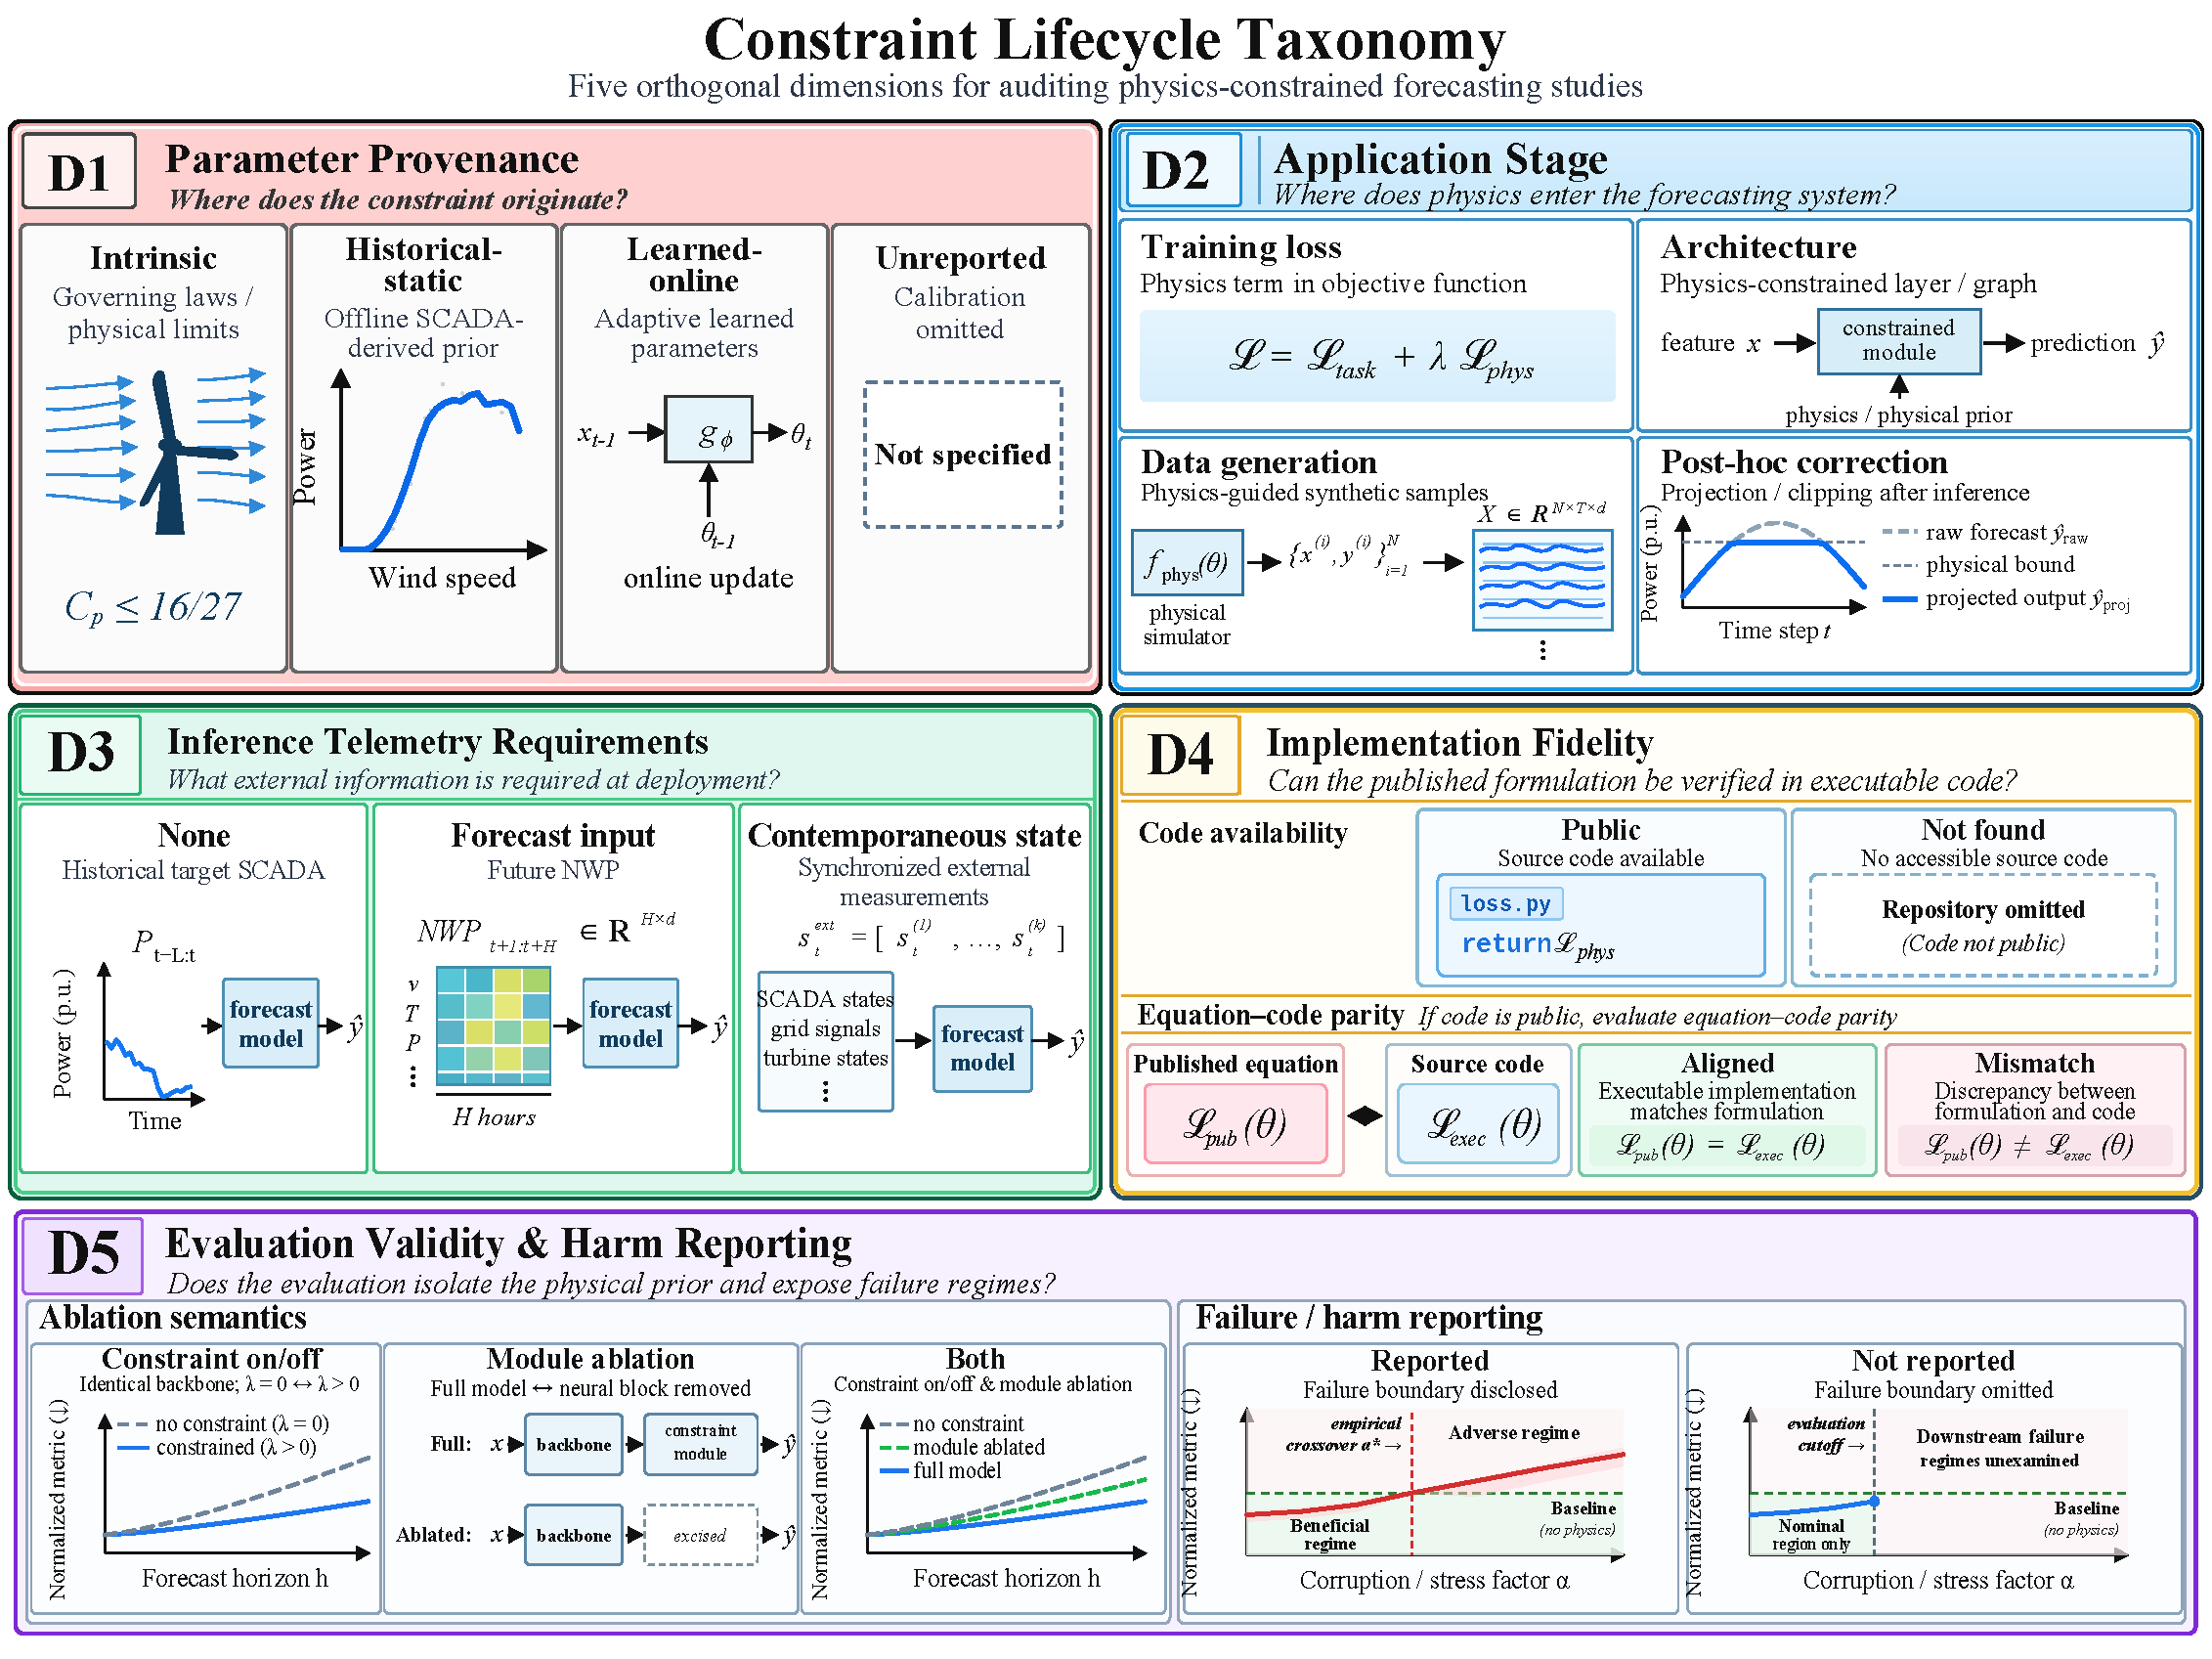
\includegraphics[width=\textwidth]{fig_constraint_lifecycle.pdf}
\caption{五维物理约束生命周期框架 (Schema v4)。系统追踪领域物理约束从数学机理来源 ($\mathcal{D}_1$)、计算图融入方式 ($\mathcal{D}_2$)、工业在线遥测依赖 ($\mathcal{D}_3$)、软件代码执行保真度 ($\mathcal{D}_4$) 到实证失效与消融有效性报告 ($\mathcal{D}_5$) 的全流程演进路径。}
\label{fig:lifecycle}
\end{figure*}

\subsection{五大生命周期维度的操作化定义}
Schema v4 通过五个正交维度对每个物理约束对象进行完备刻画：

\paragraph{维度 1：参数来源 ($\mathcal{D}_1$)}
该维度追踪约束数值参数的认识论起源与校准方式：
\begin{itemize}[leftmargin=1.5em,itemsep=1pt,topsep=2pt]
\item \textit{内生解析参数 (intrinsic)}：参数直接由第一性物理定律、出厂铭牌或经典方程推导，无需经验拟合（如 Betz 极限 $C_p \le 16/27$ 或经典运动学尾流方程）。
\item \textit{历史静态经验先验 (historical-static)}：参考曲线或分布由历史 SCADA 离线拟合并在推理中保持固定（如核密度估计经验流形）。
\item \textit{在线自适应学习参数 (learned-online)}：参数在推理期由辅助神经网络动态推断。
\end{itemize}
若文献未披露校准流程，归入\textit{未披露 (unreported)}。区分参数来源至关重要：静态经验先验隐式假定气动稳态，在机组老化或弃风限电时面临隐性失准风险。

\paragraph{维度 2：作用阶段 ($\mathcal{D}_2$)}
该维度界定物理知识介入深度学习流水线的具体计算环节：
(1)~\textit{训练损失正则化 (training-loss)}：物理先验作为可微惩罚项嵌入反向传播（$\mathcal{L} = \mathcal{L}_{\text{task}} + \lambda \mathcal{L}_{\text{phys}}$）；
(2)~\textit{推理架构约束 (inference-architecture)}：修改网络拓扑以严格限制前向输出可行域；
(3)~\textit{数据生成增强 (data-generation)}：在训练前用于合成或清洗数据；
(4)~\textit{事后投影滤波 (post-hoc-correction)}：推理完成后作为外置数学变换约束输出。

\paragraph{维度 3：推理遥测依赖 ($\mathcal{D}_3$)}
该维度识别在线部署时计算物理约束所需的外部实时数据流：
(1)~\textit{无外部依赖 (none)}：仅依赖目标机组历史功率自回归序列；
(2)~\textit{前瞻预测依赖 (forecast-input)}：必须输入未来气象预报（如数值天气预报风向风速）；
(3)~\textit{同期状态依赖 (contemporaneous-state)}：前向推理需要来自临近机组或测风塔的无延迟同步物理测量。
关键的逻辑区分在于：$\mathcal{D}_3 = \texttt{none}$ 仅界定基准预测模型本身不需要外部实时数据流（如测风塔实时遥测或前瞻数值天气预报）。然而，若某一物理约束机制在测试推理期依赖外部气象物理代理（例如利用风速输入检索经验静态功率曲线先验），而实际现场又缺乏前瞻数值天气预报或零延迟传感器时，工程部署将被迫在测试推理期剔除约束或以存在滞后的历史观测代偿。因此，观测陈旧度（observation staleness）是依赖物理代理的约束架构在现实遥测延迟下的实证运行隐患，而非 $\mathcal{D}_3 = \texttt{none}$ 分类所内生的必然推论。

\paragraph{维度 4：实现保真度 ($\mathcal{D}_4$)}
该维度评估公开软件是否忠实执行已发表论文的数学规范：
(1)~\textit{验证对齐 (verified-aligned)}：公开代码经审查证实与论文公式完全相符；
(2)~\textit{代码失配 (code-mismatch)}：公开代码在代数形式或参数方向上偏离论文公式；
(3)~\textit{未找到代码 (not-found)}：未提供公开仓库或执行脚本。
数学排版常掩盖数值执行差异，使得静态代码审计成为不可或缺的复核手段。

\paragraph{维度 5：危害报告与消融语义 ($\mathcal{D}_5$)}
该维度审查实证评估是否因果隔离了物理约束本身：
(1)~\textit{严格隔离消融 (strict-isolation)}：基准与实验组参数容量完全对齐，仅改变物理先验权重（$\lambda=0$ vs.\ $\lambda>0$）；
(2)~\textit{粗粒度模块消融 (module-ablation)}：直接切除多层神经网络子模块，混淆参数容量与领域先验；
(3)~\textit{兼具两者 (both)}：同时报告参数隔离与模块切除；
(4)~\textit{危害报告 (harm-reported)}：显式量化约束导致性能劣化的运行边界。

\subsection{消歧准则与体系形式化一致性}
为确保多位独立评分员在分类编码中达成高复现性，Schema v4 确立了三项基础消歧准则。参数来源（$\mathcal{D}_1$）严格独立于测试期遥测（$\mathcal{D}_3$）：离线标定参数所用的历史数据，与在线推理所需的实时数据流在工程上相互独立。作用阶段（$\mathcal{D}_2$）依据梯度反向传播路径进行严格判定：仅在反向传播中施加损失惩罚的归入训练期损失正则化，在网络随机初始化下仍能限制前向计算域的归入推理期架构约束。因果消融（$\mathcal{D}_5$）必须采用严格参数匹配的对照基准：直接移除多层神经网络子模块反映的是网络整体表征容量的变动，无法作为物理先验的独立因果依据。

\section{范围界定审计协议与实证测试平台}
\label{sec:protocol}

我们依据范围界定综述的 PRISMA 扩展规范（PRISMA-ScR）指南 \cite{tricco2018} 以及经典系统综述方法学 \cite{levac2010} 开展了系统审计。审计协议在全文提取前已预先明确制订，以规范检索字符串、合格性阈值、多轮筛选流程以及评分员间信度消歧。

\subsection{信息来源与文献检索策略}
文献检索覆盖 2023 年 1 月 1 日至 2026 年 3 月 1 日的时间窗口，并滚动监测至 2026 年 7 月以追踪最新预印本。首先，我们通过 OpenAlex API 开展程序化检索（该数据库全面索引 IEEE Xplore、ScienceDirect、SpringerLink、Wiley 与 MDPI）。采用四个题名布尔查询——$Q_1$ (\texttt{"physics-constrained" AND "wind"})、$Q_2$ (\texttt{"physics-informed" AND "wind power"})、$Q_3$ (\texttt{"physics-guided" AND "wind"}) 与 $Q_4$ (\texttt{"physics-embedded" AND "wind power"})——初筛召回 72 项候选记录。其次，针对 Google Scholar、arXiv 与预印本服务器开展靶向检索，补充捕获 17 项在线发表期刊与工作论文，初始候选文献总量达 $N=89$ 项。召回文献与 Scopus 及 IEEE Xplore 进行了交叉核验，以保证对能源与人工智能核心期刊的充分覆盖。全部检索式、原始记录与排除日志均归档于开源补充数据台账中。此外，我们将检索字段拓展至 Scopus 与 IEEE Xplore 题名、摘要与关键词（包含 \texttt{"knowledge-guided"}、\texttt{"hybrid"} 与 \texttt{"domain-informed"} 等更宽泛术语）开展了定向敏感性检索，额外识别出 14 篇文献；全文审查确认其中无一报告失效工况或负面权衡，专门用于压力测试 0.0\% 负面权衡结论的稳健性。需强调的是，这 14 篇敏感性文献专门用于核验负面危害报告；完整的五维（$\mathcal{D}_1$--$\mathcal{D}_5$）深度提取与评分员间信度检验严格在由 PRISMA-ScR 规范确立的核心 46 项研究语料库中开展。

\begin{figure}[!t]
\centering
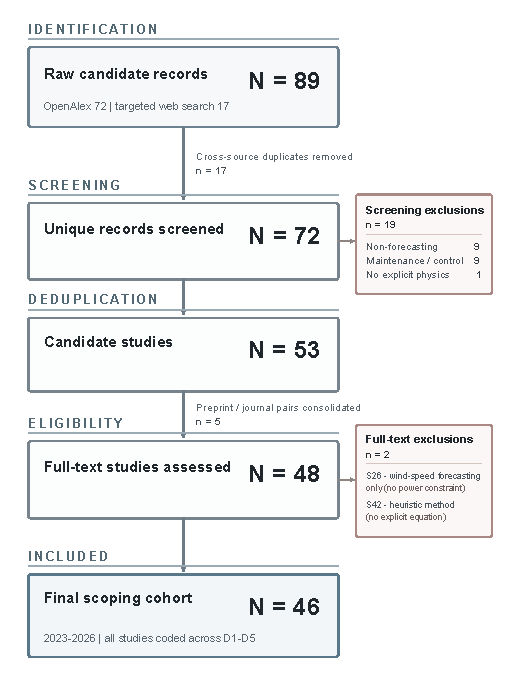
\includegraphics[width=\columnwidth]{prisma_flow_diagram.pdf}
\caption{PRISMA-ScR 范围界定语料库推导流程图 ($89 \rightarrow 72 \rightarrow 53 \rightarrow 48 \rightarrow 46$)。跨源去重消除了17项重复记录，预印本-期刊成对合并去重归并了5项，全文资格审查排除了2项，最终确定 46 项合资格全文研究。}
\label{fig:prisma_flow}
\end{figure}

\subsection{文献筛选、去重与纳入排除准则}
候选记录经历了如图~\ref{fig:prisma_flow}所示的多阶段结构化筛选。跨数据库查重从初始的 89 项记录中剔除了 17 项重复条目，保留 72 项独立记录进入题名与摘要评估。该阶段依据明确标准排除了 19 项记录：9 项聚焦于非预测类任务（如风机结构健康监测、叶片裂纹检测或气弹疲劳损伤建模）；9 项专注于毫秒/秒级实时变桨与有功功率控制而非多步功率预测；1 项不包含任何物理融入建模组件。此阶段最终筛选出 53 项待检索全文的研究。

由于作者在正式期刊录用前通常在公开预印本库（如 arXiv 或 SSRN）发布初稿，将同一课题的预印本与正式期刊论文割裂看待会人为虚增文献统计基数。为此，我们执行了严格的“研究级”（Study-level）成对合并去重准则：只要预印本与已发表同行评审期刊论文共享完全相同的作者群、实证数据集与核心数学公式，两者即被合并为单项研究台账，统一保留正式期刊引用。经过细致比对，共识别并合并了 5 对重复条目（例如 \textit{Applied Energy} 2025 与 SSRN 2024；\textit{Electric Power Systems Research} 2026 与 SSRN 2026），将候选集精炼至 48 项独立研究。

对其余 48 篇全文文献，两名审计员依据三项明确的范围界定合格性准则进行了独立评估：(1) 研究核心聚焦于超短期或短期风电功率预测；(2) 明确形式化构建并在计算中执行了显式物理约束、控制方程或领域边界；(3) 在真实或仿真风电功率时间序列上开展了实证评估。审查最终排除了 2 项研究：研究 S26 仅预测大气风速而未施加风电功率约束；研究 S42 仅实现了启发式特征子空间聚类而无任何领域物理方程。此番严格筛选确立了最终符合 PRISMA-ScR 规范的代表性实证审计文献库，共包含 \textbf{$N=46$ 项独立研究}（涵盖 38 篇同行评审期刊论文与 8 篇具有广泛影响力的预印本/工作论文，包括 UniWind \cite{s27_uniwind2026}）。

\subsection{评分员间信度基准测试}
为在全语料库数据提取前验证 Schema v4 分类体系的操作稳定性，三名独立评分员（Coder A、Coder B 与 Coder C）对分层抽样的 20 篇代表性文献样本进行了双盲独立编码。基准测试显示出各维度高度的评分员间一致性：文献合格性筛选达成百分之百共识（Fleiss $\kappa = 1.000$），精准剔除了对照组 S26 与 S42；参数来源（$\mathcal{D}_1$）在总体与纳入样本上均呈现完美一致性（$\kappa = 1.000$）；作用阶段（$\mathcal{D}_2$）达到近乎完美的一致性（总体 $\kappa = 0.950$，纳入样本 $\kappa = 0.938$）；推理遥测依赖（$\mathcal{D}_3$）呈现出实质性一致（总体 $\kappa = 0.743$，纳入样本 $\kappa = 0.646$）。

相比之下，实现保真度（$\mathcal{D}_4$）在仲裁前的一致性呈现中等水平（总体 $N=20$ 先导样本含负对照时 $\kappa = 0.716$，但严格在纳入样本上时下降至 $\kappa = 0.341$）。这一数值降幅在测量学与统计学中极为典型，反映了著名的 Feinstein 与 Cicchetti 患病率悖论（Prevalence Paradox）：由于纳入样本中高达 92.6\% 的文献未提供公开代码，随机期望一致率极高（$P_e = 86.1\%$），使得即使实际观测一致率高达 $P_o = 90.7\%$，计算出的 Fleiss' $\kappa$ 依然被大幅压低。此外，在缺乏公开代码仓的静态文本阅读中，不同评审员极易对正文宣称的物理约束究竟是“可执行算法”还是“概念性愿景”产生分歧，这一模糊性直接证明了仅凭正文无法可靠推断软件实现，强力支撑了开展底层静态计算图审计的方法学必要性。对于消融语义（$\mathcal{D}_5$），评分员达成高度一致（总体 $\kappa = 0.851$，纳入样本 $\kappa = 0.818$）；而在危害报告方面，三位评分员在 18 篇纳入文献中均一致判定危害报告为零（0/18），由于无边际方差（$P_e = 1.0$），Kappa 统计量在数学上未定义，严格报告为 100\% 观测一致率（$P_o = 1.000$）。在完成先导校准与仲裁一致后，全量 46 篇文献由第一作者（J.L.）完成逐行全文提取并记录精准章节、公式编号与原文证据，并由第二作者（J.D.）对核心定量参数进行独立复核。

\subsection{软件代码审计协议 (PCT 与 PINN-UQ)}
软件可用性审计遵循标准化的五阶段检索流程，全面排查正文主体、脚注、数据与代码可用性声明、出版社公开代码托管库以及作者学术主页。在全量 46 项研究中，仅有两篇论文提供了公开可获取的代码库。其中，PINN-UQ (S10, \textit{Eng. App. AI} 2025) 经审计确认其计算图严格忠实实现了其所陈述的机电代数方程（通过 \texttt{sn.Tie} 实现 $P = g T \omega$ 与 $P = \frac{1}{2} C_p \rho A v^3$），分类为\textit{验证对齐}。另一公开项目物理约束 Transformer (PCT, S02, \textit{Sci. Rep.} 2026) 提供了官方 GitHub 仓库（提交哈希 \texttt{65941ec}），我们对其核心训练脚本（\texttt{train\_clean.py} 和 \texttt{tst/loss.py}）开展了逐行计算图与抽象语法树审计，具体细节见第~\ref{sec:code_audit}节。

\subsection{下游电力系统实际调度与出清结算实证测试基准}
为使实证审计扎根于跨越异质微地形的真实电力系统运行，我们在英国三座商业级陆上风电场（具备10分钟级高精度工业SCADA遥测）上搭建了前瞻性实证测试平台。\textit{Hill of Towie 风电场}（额定装机 48.3~MW，21 台西门子 SWT-2.3-82 机组）地处复杂起伏高地，微地形尾流干扰显著，作为独立时空外推基准（全量 2017 年 7,599 个滚动预报起点，对应 45,594 个下步结算时段），该数据集由 RES 代表 TRIG 在 Zenodo 上以 CC-BY-4.0 许可开源发布 \cite{zenodo_hilloftowie}。\textit{Kelmarsh 风电场}（额定装机 12.3~MW，6 台森吉安 MM92 机组）位于开阔平原农田，作为核心开发基准（8,212 个预报起点，49,272 个结算时段）\cite{zenodo_kelmarsh}。\textit{Penmanshiel 风电场}（额定装机 28.7~MW，14 台森吉安 MM82 机组，编号 WT01--WT15，其中 WT03 缺省）\cite{zenodo_penmanshiel} 位于苏格兰边境丘陵地带，具有 8,440 个预报起点，我们配置了样本受限分区（$N_{\text{train}} = 1,583$），用于测试小样本受限工况下的过拟合与物理先验引导能力。需特别强调的是，由于 Penmanshiel 在地形与机型上与 Kelmarsh 及 Hill of Towie 均存在固有物理差异，跨站点对比必然同时叠加了地形异质性与样本量差异，因此必须依赖场站内受控消融实验以严密隔离样本规模因素。

测试基准在严格冻结的前瞻性协议下运行：输入历史回溯长度 $L=36$（6小时），预测时域 $H=36$（6小时），下游日前调度考核关注次小时交付窗口 $H_{\text{disp}} = \{1, \dots, 6\}$，滚动步长 $S=6$ 以避免相邻结算周期重叠。基准模型套件涵盖无约束 DLinear、边界约束 DLinear ($\lambda=0.01$)、经验功率曲线约束 DLinear ($\lambda=0.01$)、经验条件分布先验 DLinear ($\lambda=0.01$)，并引入经典 Ridge 岭回归与 Persistence 持续性预测作为基准，均在 5 个随机初始化种子下重复评估。此外，为验证发现是否受限于线性结构，我们额外引入了代表性多块通道独立 Transformer 架构（\textbf{PatchTST} \cite{nie2023patchtst}，块长度6，步长4，隐藏维度64，带RevIN的两层编码器），在三座风场、四种约束配置与5个种子下完成 60 次独立训练运行，作为探索性深度架构敏感性基准。

离线决策校准采用后验分位数偏移标定 $\delta_h$，参数严格在独立的 2016 年校准集上拟合（在罚款比率 $r=2$ 下对应临界分位数 $q = 1/(r+1) = 1/3$），对 2017 年测试期 SCADA 与市场价格实现严格盲化。真实市场出清基于英国 Elexon BSC 2017 全年官方系统买入价格（SBP，均值 \pounds 44.27/MWh，峰值 \pounds 1,509.80/MWh，包含 68 个下探至 -\pounds 73.15/MWh 的负电价时段）。结算严格执行 30 分钟物理净偏差结算规则：
\begin{equation}
E_{SP} = \sum_{t \in SP} (p_t - y_t) \cdot \frac{P_{\text{rated}}}{6000} \quad [\text{MWh}],
\label{eq:bsc_netting}
\end{equation}
由此生成单边短缺清算惩罚与双边不平衡结算现金流作为决策风险诊断，所有统计显著性均通过 2,000 次 7 天圆形块成对自举检验（Block Bootstrap）予以严密核验。

\section{实证审计结果}
\label{sec:results}

涵盖 46 项范围界定文献与三座商业风电场前瞻受控消融基准的实证审计，系统裁决了物理约束风电预测的核心运行主张。

\subsection{审计文献中运行失效边界的系统性缺失}
对 46 项核心范围界定文献的审计表明，已发表论文无一记录运行负面权衡或约束失效工况（0.0\%，46/46，95\% Wilson 置信区间：[92.3\%, 100.0\%]，\texttt{negative\_effect == 'no'}）。这一零负面效应报道特征在我们针对 Scopus 与 IEEE Xplore 扩展检索字段（包含 knowledge-guided、hybrid 与 domain-informed 等宽泛词汇）的 14 篇补充敏感性检索中同样得到确认。在核心语料库中，仅 3 项研究（6.5\%，S01、S02、S10）评估了先验参数扰动，其余 43 项研究（93.5\%）均仅在理想标称工况下测试。标称工况下的单一报道掩盖了工程折中与有效性边界，以普适提升的叙事替代了严谨的工程边界界定。

\subsection{严峻的公开代码赤字严重阻碍独立验证}
在 46 项核心研究中，静态软件审计确立了高达 95.7\% 的公开代码赤字（44/46，95\% Wilson 置信区间：[85.5\%, 98.8\%]，$\mathcal{D}_4 = \texttt{not-found}$），44 篇论文既未提供公开代码仓库亦未提供可执行脚本。在仅有的两个公开代码库中，PINN-UQ (S10) 提供了经静态审查证实与其机电代数方程完全对齐的可执行代码（$\mathcal{D}_4 = \texttt{code-aligned}$，2.2\%）；而作为端到端物理约束 Transformer 唯一公开训练代码库的 PCT (S02)，在核心损失函数的执行方向上与发表论文存在代数级失配（$\mathcal{D}_4 = \texttt{divergent-code}$，2.2\%）。被审计文献中 97.8\% 的研究因此无法开展独立的计算复核。

\subsection{约束生命周期分布与消融实验的结构混淆}
消融语义审计（$\mathcal{D}_5$）揭示出核心语料库中半数文献存在结构性因果混淆：50.0\% 的研究（23/46，95\% Wilson 置信区间：[36.1\%, 63.9\%]）通过直接移除多层神经网络子模块（如空间图卷积层、交叉注意力块或模态分解单元）开展消融，而非隔离惩罚权重（$\lambda=0$ vs. $\lambda>0$）。剥离网络模块同步移除了成千上万个可训练参数，所测得的性能差异反映的是网络综合表征容量而非物理先验本身（表~\ref{tab:lifecycle_distribution}，图~\ref{fig:audit_distribution}）。需要特别强调的是，上述公开代码赤字（95.7\%）与粗粒度模块消融（50.0\%）统计比例严格限定于本研究系统审计的 46 项核心文献语料库及其 Wilson 置信区间，避免无边界外推至所有可能替代关键词文献。

\begin{table*}[!t]
\centering
\footnotesize
\renewcommand{\arraystretch}{0.92}
\setlength{\tabcolsep}{3.5pt}
\caption{46 项审计文献中物理约束生命周期维度的经验分布统计 (2023--2026)。}
\label{tab:lifecycle_distribution}
\begin{tabularx}{\textwidth}{p{3.6cm}p{3.0cm}rrX}
\toprule
\textbf{生命周期维度} & \textbf{分类子类} & \textbf{文献数量 ($N=46$)} & \textbf{占比 (\%)} & \textbf{审计文献中的典型代表案例} \\
\midrule
\multirow{3}{*}{\textbf{D1: 参数来源}} 
& \texttt{内生解析参数} & 40 & 87.0\% & Betz 气动理论极限 ($C_p \le 16/27$)、额定装机容量 $P_{\text{rated}}$、Jensen 尾流模型 \\
& \texttt{历史静态先验} & 5 & 10.9\% & 双变量经验功率曲线 ($P=f(v)$)、在训练集 SCADA 上离线估计的 2D KDE 分布 \\
& \texttt{在线自适应学习} & 1 & 2.2\% & 辅助子网络动态预测在线时变气动系数 $C_p(t)$ \\
\midrule
\multirow{4}{*}{\textbf{D2: 作用阶段}} 
& \texttt{训练期损失正则化} & 21 & 45.7\% & 反向传播中的可微惩罚项 ($\mathcal{L} = \mathcal{L}_{\text{MSE}} + \lambda \mathcal{L}_{\text{phys}}$) \\
& \texttt{推理期计算架构} & 23 & 50.0\% & 尾流引导的 GNN 邻接矩阵、单调激活函数层、双流物理特征融合网络 \\
& \texttt{上游数据生成} & 1 & 2.2\% & 物理引导的扩散生成模型合成极端风电出力场景 \\
& \texttt{事后修正投影} & 1 & 2.2\% & 推理完成后的外置保形预测校正与物理可行域流形投影层 \\
\midrule
\multirow{3}{*}{\textbf{D3: 推理遥测需求}} 
& \texttt{无外部依赖} & 36 & 78.3\% & 标准历史自回归 SCADA 序列；运行时零外部前向数据流依赖 \\
& \texttt{前瞻气象预报依赖} & 6 & 13.0\% & 必须依赖未来预测时段 $[t+1, t+H]$ 内的 NWP 数值天气预报输入 \\
& \texttt{同期空间遥测依赖} & 4 & 8.7\% & 必须依赖来自相邻机组或测风塔的同步无延迟现场 SCADA 测量 \\
\midrule
\multirow{3}{*}{\textbf{D4: 实现保真度}} 
& \texttt{未找到公开代码} & 44 & 95.7\% & 在既定审计检索协议下未发现任何公开可访问的代码仓库或复现脚本 \\
& \texttt{代码失配} & 1 & 2.2\% & PCT: 损失函数底层执行反向参数 JS 散度而非论文声明的标准 JS 散度 \\
& \texttt{验证对齐} & 1 & 2.2\% & PINN-UQ: 机电代数代数约束经底层审查证实与论文公式严格保真对齐 \\
\midrule
\multirow{3}{*}{\textbf{D5: 评估有效性与危害报告}} 
& \texttt{组件级消融} & 23 & 50.0\% & 整体切除多层神经网络子模块；混淆网络参数容量与物理归纳偏置 \\
& \texttt{约束开闭消融} & 17 & 37.0\% & 在严格相同的网络容量下切换惩罚项权重 ($\lambda=0$ vs.\ $\lambda>0$) \\
& \texttt{两者兼备} & 6 & 13.0\% & 在对比基线中同时执行参数切换与架构消融 \\
\bottomrule
\end{tabularx}
\end{table*}


\begin{figure*}[!t]
\centering
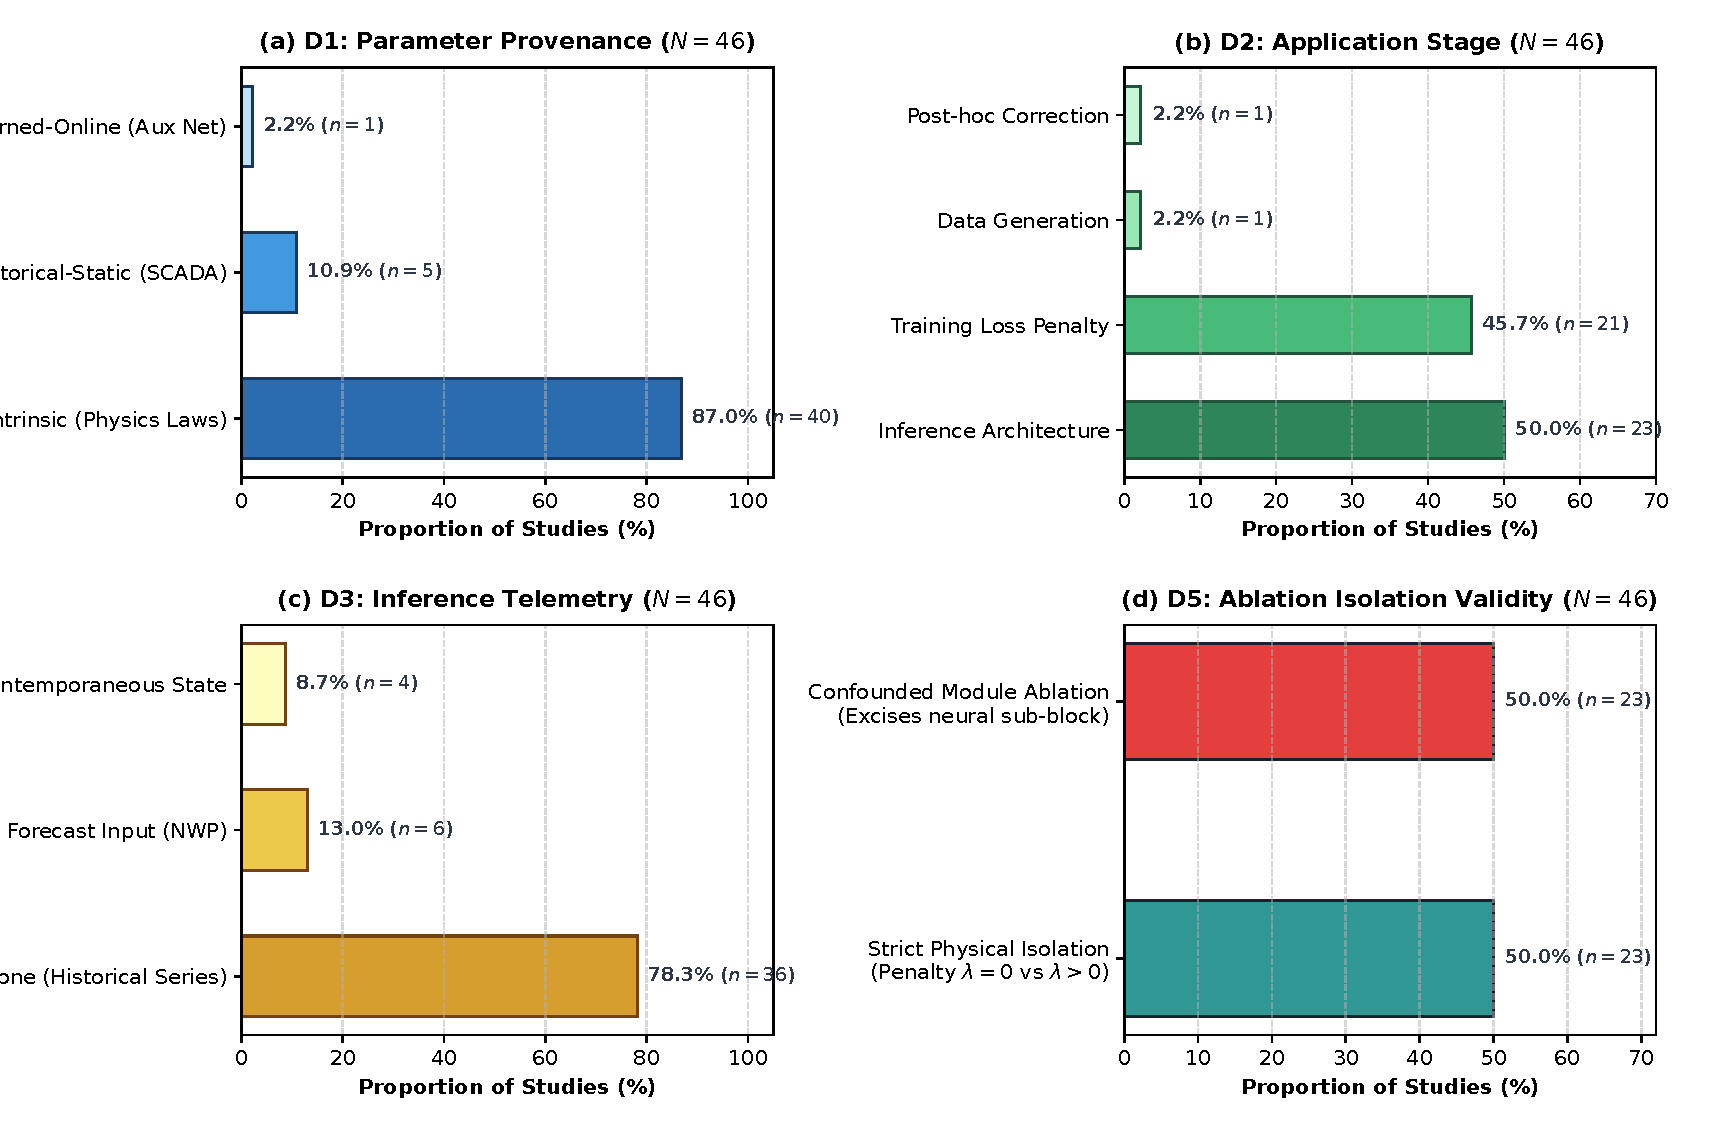
\includegraphics[width=\textwidth]{fig_field_audit_distribution.pdf}
\caption{46 项审计文献的生命周期经验分布 ($N=46$)。(a) $\mathcal{D}_1$ 参数来源；(b) $\mathcal{D}_2$ 作用阶段；(c) $\mathcal{D}_3$ 推理遥测需求；(d) $\mathcal{D}_5$ 消融语义细分（严格物理隔离消融 vs 混淆的多参数模块级消融）。}
\label{fig:audit_distribution}
\end{figure*}

\subsection{因果解耦：先验误设敏感性、数值正则化拟态与静态代理陈旧度}
三座商业级风电场的 3D 前瞻受控消融实验隔离了先验误设、数值平滑与静态观测陈旧度的因果效应（表~\ref{tab:controlled_ablation}，图~\ref{fig:causal_ablation}）。

\begin{table*}[!t]
\centering
\footnotesize
\renewcommand{\arraystretch}{0.82}
\setlength{\tabcolsep}{3.5pt}
\caption{3D 前瞻性受控消融实验基准：物理知识特异性、数值平滑拟态与滞后代理衰减在三座风电场上的因果解耦（多随机种子评估，分位数决策校准 $r=2, q=1/3$）。}
\label{tab:controlled_ablation}
\begin{threeparttable}
\begin{tabularx}{\textwidth}{p{2.2cm}p{3.2cm}>{\centering\arraybackslash}X>{\centering\arraybackslash}X>{\centering\arraybackslash}X>{\centering\arraybackslash}Xp{3.8cm}}
\toprule
\textbf{风电场站点} & \textbf{受控实验分支} & \textbf{归一化调度成本} & \textbf{Pinball 损失} & \textbf{RMSE} & \textbf{短缺清算支出} & \textbf{因果作用机理} \\
\textbf{\& 地形地貌} & \textbf{(消融测试工况)} & \textbf{$\text{Cost}_{static}$ ($r=2$)} & \textbf{($q=1/3$)} & \textbf{(标幺值)} & \textbf{(\pounds/(台$\cdot$年))} & \textbf{\& 实证结论} \\
\midrule
\multirow{6}{=}{\textbf{Kelmarsh}\\(12.3 MW, 6台机)\\\textit{开阔平原地貌}\\\textit{$N_{train}=5,098$}} 
& 纯数据无约束基准 & $0.08812 \pm 0.00009$ & 0.02937 & 0.1717 & \pounds 5,831.79 & 纯功率自回归 baseline \\
& 信息对称特征增强 (功率+风速) & $0.08910 \pm 0.00039$ & 0.02970 & 0.1697 & \pounds 5,982.26 & 同期风速轻微优化 RMSE 但抬高尾部决策成本 \\
& 真实经验功率曲线 ($\lambda=0.1$) & \textbf{$0.08791 \pm 0.00009$} & \textbf{0.02930} & 0.1708 & \pounds 5,780.99 & 真实物理下行保护 ($-0.24\%$) \\
& 伪打乱经验先验 ($\lambda=0.01$) & $0.08801 \pm 0.00008$ & 0.02934 & 0.1724 & \pounds 5,657.03 & \textbf{与真实先验统计不可区分}；低 $\lambda$ 实证表现为非特异性数值正则化 \\
& 真实经验联合分布 ($\lambda=0.1$) & $0.09841 \pm 0.00085$ & 0.03280 & 0.1703 & \textbf{\pounds 8,412.28} & \textbf{显著运行负面损伤}：平原工况下短缺罚款激增 $+44.2\%$ \\
& 滞后遥测代理扫描 ($k=36$, 6h) & $0.09043 \pm 0.00006$ & 0.03014 & 0.1729 & \pounds 5,888.58 & 随陈旧风速代理延迟呈现单调性能恶化 \\
\midrule
\multirow{6}{=}{\textbf{Hill of Towie}\\(48.3 MW, 21台机)\\\textit{复杂起伏山地}\\\textit{$N_{train}=7,035$}} 
& 纯数据无约束基准 & $0.08924 \pm 0.00005$ & 0.02975 & 0.1740 & \pounds 6,006.09 & 鲁棒的无约束对比基准 \\
& 信息对称特征增强 (功率+风速) & $0.09042 \pm 0.00007$ & 0.03014 & 0.1733 & \pounds 6,297.16 & 高频风速噪声放大日前申报决策方差 \\
& 真实经验功率曲线 ($\lambda=0.1$) & \textbf{$0.08916 \pm 0.00007$} & \textbf{0.02972} & 0.1745 & \pounds 5,958.34 & 次小数位边际改善 ($-0.09\%$) \\
& 伪打乱经验先验 ($\lambda=0.01$) & $0.08919 \pm 0.00006$ & 0.02973 & 0.1740 & \pounds 6,069.01 & 确认低惩罚尺度下的非特异性数值正则化行为 \\
& 真实经验联合分布 ($\lambda=0.1$) & $0.09503 \pm 0.00022$ & 0.03168 & 0.1801 & \pounds 5,702.68 & \textbf{指标反转}：现金流增至1.2万镑但实际决策成本恶化 $+6.5\%$ \\
& 滞后遥测代理扫描 ($k=36$, 6h) & $0.09257 \pm 0.00007$ & 0.03086 & 0.1759 & \pounds 6,281.82 & 物理代理陈旧度单调蚕食物理先验的指引价值 \\
\midrule
\multirow{6}{=}{\textbf{Penmanshiel}\\(28.7 MW, 14台机)\\\textit{波状丘陵微地形}\\\textit{$N_{train}=1,583$ (匮乏)}} 
& 纯数据无约束基准 & $0.09881 \pm 0.00027$ & 0.03294 & 0.2058 & \pounds 6,713.83 & 小样本匮乏工况，模型面临严重过拟合 \\
& 信息对称特征增强 (功率+风速) & $0.10461 \pm 0.00005$ & 0.03487 & 0.2091 & \pounds 6,630.38 & 盲目增加入网特征在小样本下加剧表示发散 \\
& 真实经验功率曲线 ($\lambda=1.0$) & \textbf{$0.09760 \pm 0.00044$} & \textbf{0.03254} & 0.2054 & \pounds 6,808.40 & \textbf{扎实的物理归纳护栏收益} ($-1.22\%$) \\
& 伪打乱经验先验 ($\lambda=1.0$) & $0.16611 \pm 0.00335$ & 0.05537 & 0.2384 & \textbf{\pounds 11,561.19} & \textbf{物理特异性实证确立}：打乱物理映射导致严重性能劣化 ($+68.1\%$) \\
& 真实经验联合分布 ($\lambda=0.01$) & $0.09833 \pm 0.00027$ & 0.03278 & 0.2055 & \pounds 6,543.36 & 小样本下提供稳定的防御性正则化效果 \\
& 滞后遥测代理扫描 ($k=36$, 6h) & $0.10473 \pm 0.00036$ & 0.03491 & 0.2083 & \pounds 7,090.86 & 第 36 步滞后彻底抵消物理先验所有相对增益 \\
\bottomrule
\end{tabularx}
\begin{tablenotes}[flushleft]
\footnotesize
\item \textbf{注记}：(1) 模型在 10 卡物理 GPU 集群上评估：Kelmarsh 采用 4 个随机种子 (42--45)；Hill of Towie 与 Penmanshiel 各采用 3 个随机种子 (42--44)。指标报告测试集上的“均值 $\pm$ 种子标准差”。惩罚系数网格 $\lambda \in \{0.01, 0.1, 1.0\}$ 为预设敏感性与应力测试网格；超参数与校准偏移严格在 2016 年验证与标定集选定，2017 年测试集仅在协议冻结后访问。(2) $\text{Cost}_{static} = 3 \times \text{PinballLoss}(q=1/3)$，基于验证集后验分位数偏移校准标定 ($\delta^*$)。(3) 伪打乱分支置换风速与功率的经验映射，保持完全相同的损失形式、网络架构与正则化权重 $\lambda$。(4) 滞后代理扫描对训练损失惩罚项中检索先验的历史风速施加 $k \in \{6, 12, 18, 36\}$（1 至 6 小时）的滞后，评估在缺失前向数值天气预报时训练目标对历史气象代理时效错配的敏感性。
\end{tablenotes}
\end{threeparttable}
\end{table*}


\begin{figure*}[!t]
\centering
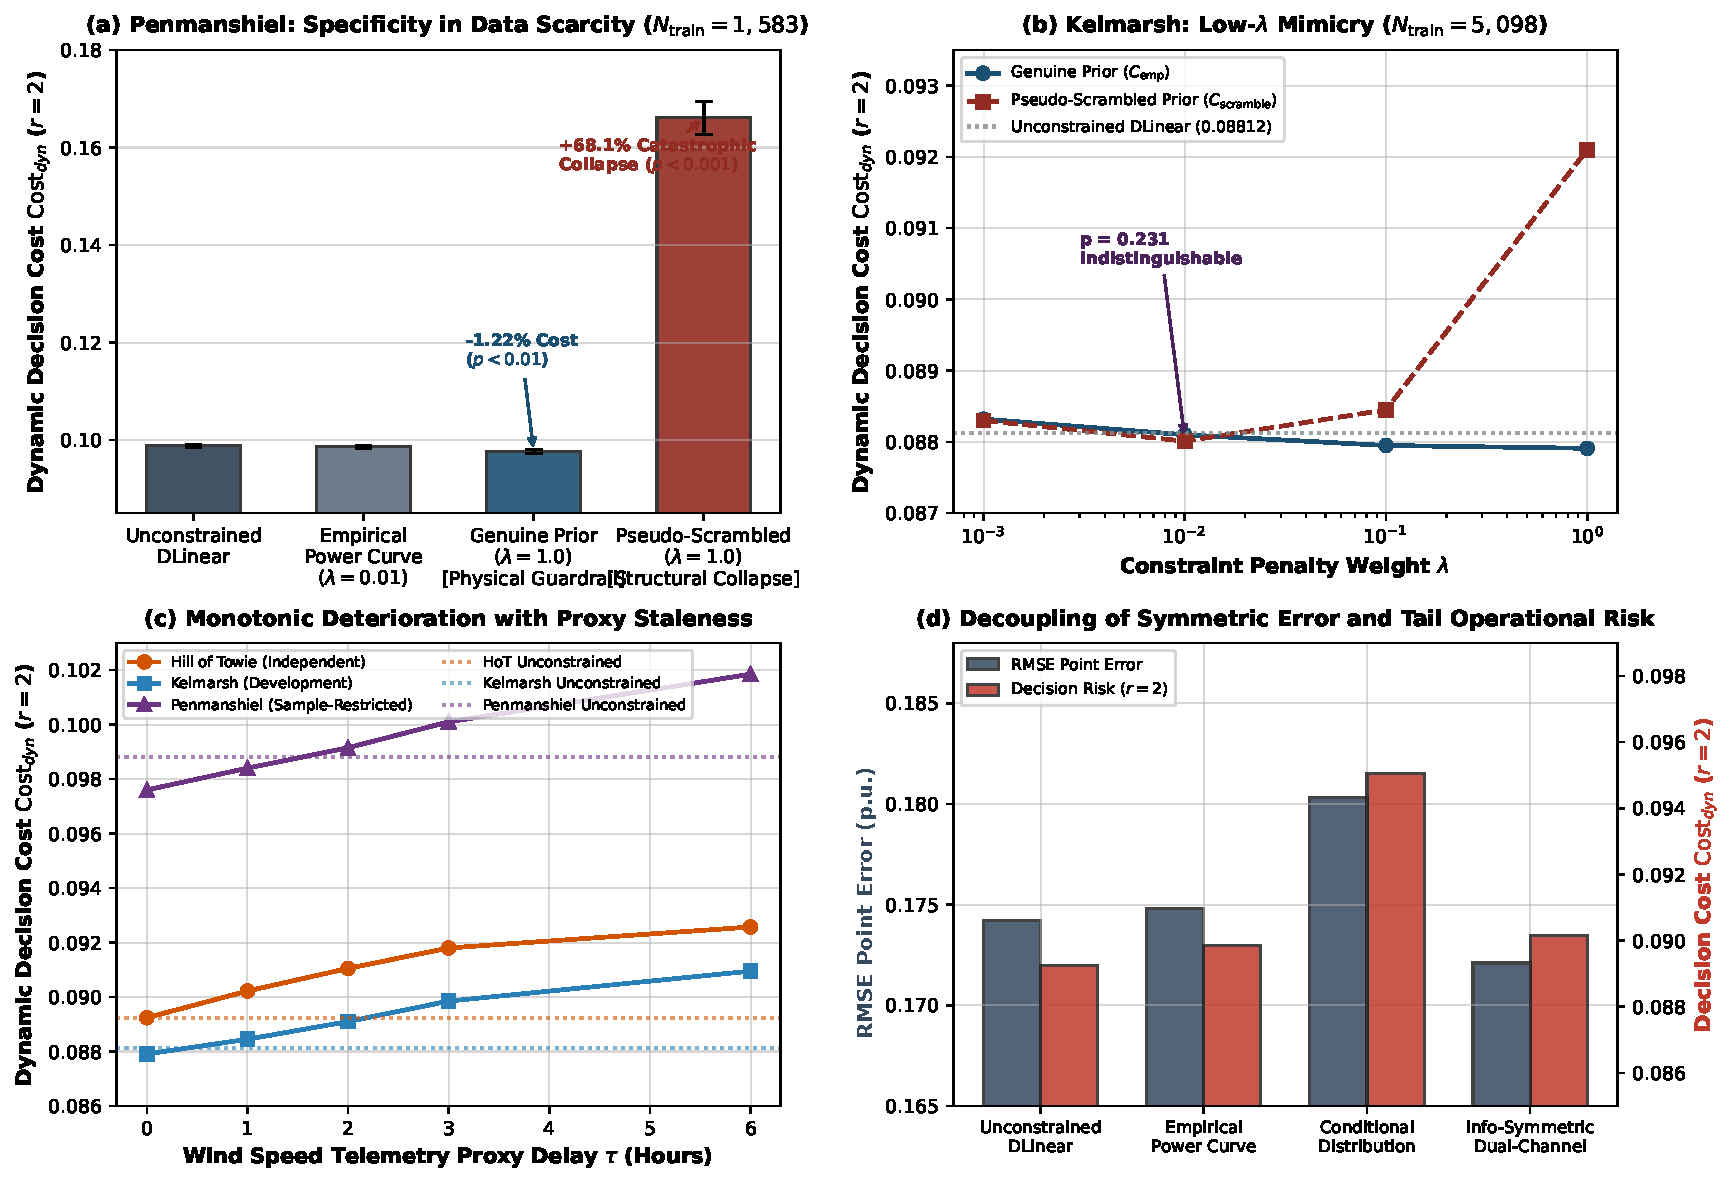
\includegraphics[width=\textwidth]{fig_causal_ablation.pdf}
\caption{三座商业级风电场的前瞻性受控消融基准实验。(a) 强物理约束对先验误设的极端敏感性（Penmanshiel 风电场，$N_{\text{train}}=1,583$）：真实物理先验带来下行风险对冲（$-1.22\%$），而破坏气动映射的伪打乱先验导致调度成本激增 $+68.1\%$；(b) Kelmarsh 风电场上的低 $\lambda$ 数值正则化拟态，在 $\lambda \le 0.01$ 时真实先验与伪打乱先验决策成本高度接近，表明弱约束在实证上更符合非特异性数值平滑而非领域物理推理；(c) 训练代理时效错配诱发的成本单调膨胀：随着训练损失中历史风速代理滞后 $k$ 从 1h 增加至 6h，三座风场的调度成本均呈单调上升；(d) 对称均方误差 (RMSE) 与非对称调度决策风险 ($r=2$) 的明显解耦，表明对称点指标掩盖了尾部运行风险。}
\label{fig:causal_ablation}
\end{figure*}

\begin{figure*}[!t]
\centering
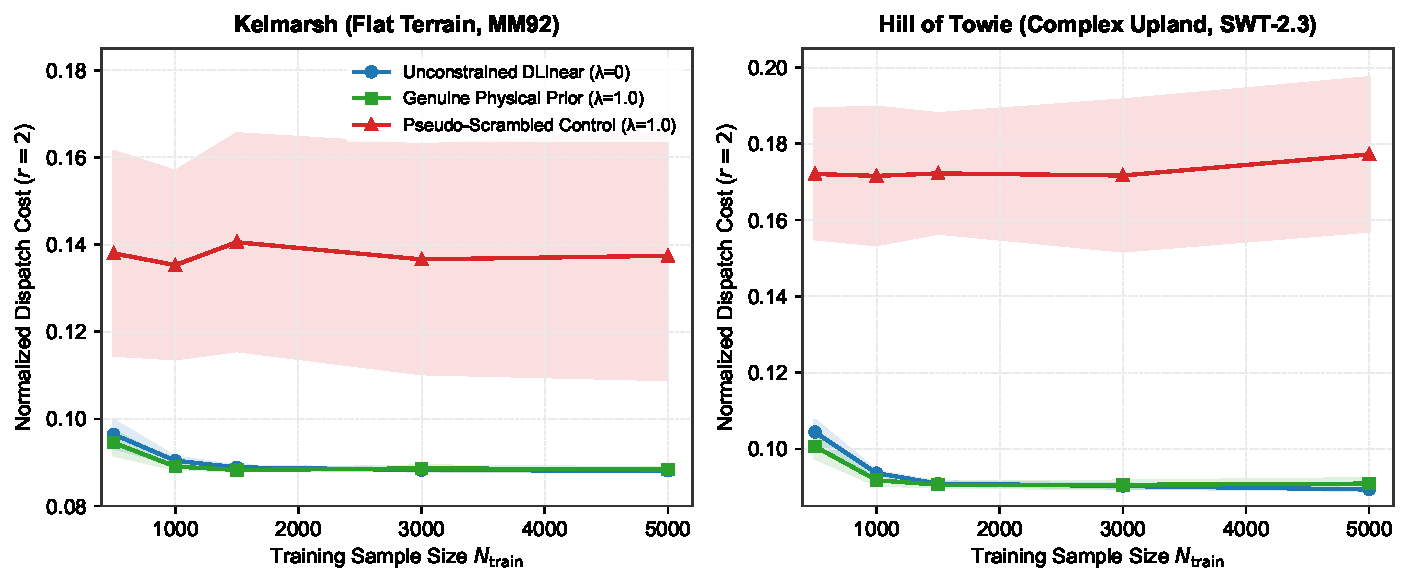
\includegraphics[width=\textwidth]{fig_within_site_learning_curve.pdf}
\caption{Kelmarsh 与 Hill of Towie 场站内样本量学习曲线（$N_{\text{train}} \in \{500, 1000, 1500, 3000, 5000\}$，多随机种子均值与标准差）。场站内实验剥离了地形与样本量的混杂：在模型受限训练窗口下（$N_{\text{train}} \le 1,000$），固定历史经验先验在两场站均取得更低的平均调度成本（Kelmarsh 降低 $-2.00\%$，Hill of Towie 降低 $-3.62\%$）；随着模型训练窗口扩大至 $N_{\text{train}}=5,000$，该优势消退并发生轻微反转（Kelmarsh 升高 $+0.33\%$，Hill of Towie 升高 $+1.73\%$）。而在强正则化（$\lambda=1.0$）下，误设的打乱先验在所有样本规模下均造成严重损害（调度成本激增 $+43\%$ 至 $+98\%$）。}
\label{fig:within_site_learning_curve}
\end{figure*}

\begin{figure*}[!t]
\centering
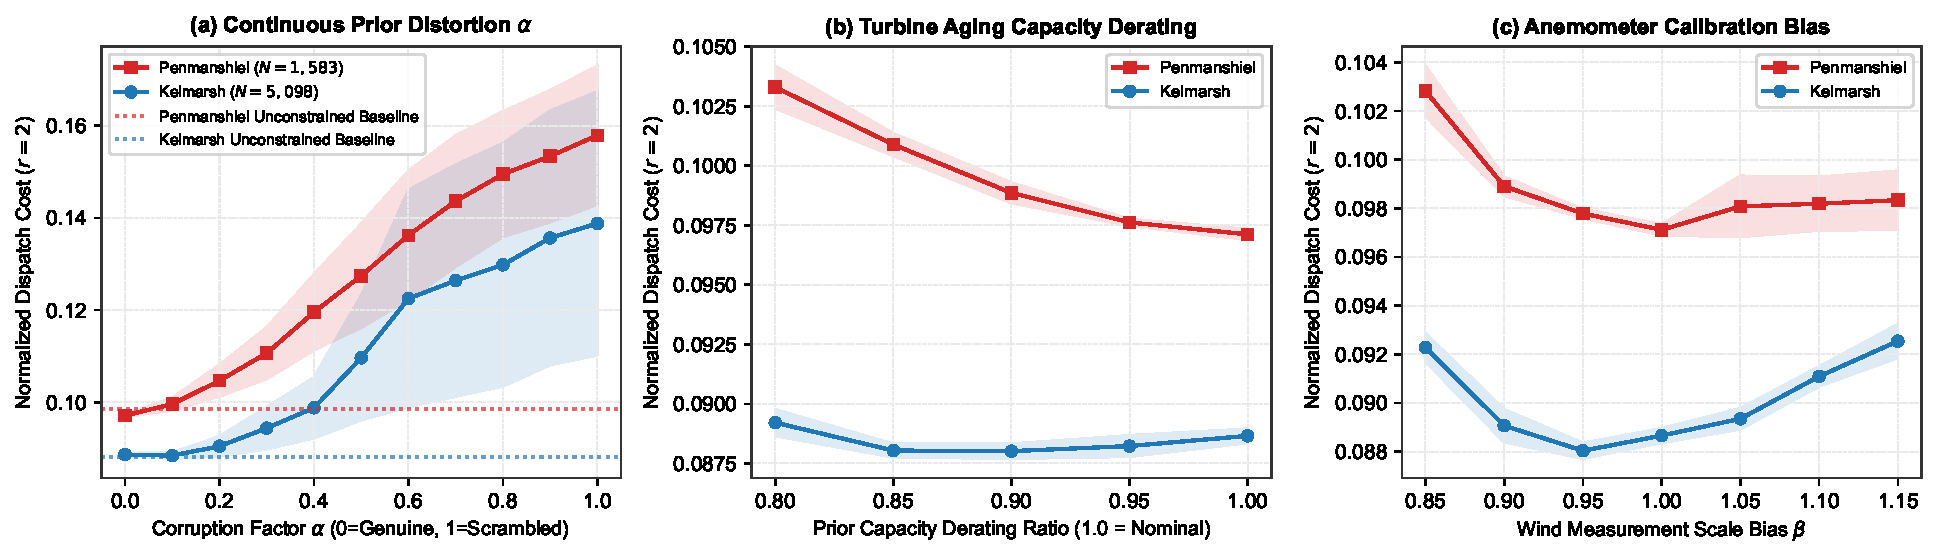
\includegraphics[width=\textwidth]{fig_prior_corruption_gradient.pdf}
\caption{连续先验退化与工程漂移敏感性响应曲面。(a) 真实先验与打乱先验的连续插值 $\alpha \in [0.0, 1.0]$，测定 Penmanshiel 上临界容错阈值约为 $\alpha^* \approx 0.07$；(b) 机组气动老化额定容量折损：折损超过 10\% 即导致先验劣于无约束基准；(c) 风速计传感器标定漂移：Penmanshiel 在正向风速偏差达 $+15\%$ 内仍能维持微弱优势，而负向低估则系统性加剧短缺惩罚。}
\label{fig:corruption_gradient}
\end{figure*}

表~\ref{tab:controlled_ablation} 与图~\ref{fig:causal_ablation} 揭示了四项实证运行边界条件：

\paragraph{防御性归纳偏置与先验误设脆弱性 (图~\ref{fig:causal_ablation}a, 图~\ref{fig:within_site_learning_curve}, 图~\ref{fig:corruption_gradient})}
在样本受限的 Penmanshiel 风电场（$N_{\text{train}} = 1,583$），无约束 DLinear 表现出过拟合（$0.09881 \pm 0.00027$）。施加校准的真实经验功率曲线先验（$\lambda=1.0$）时，归一化调度成本降至 $0.09760 \pm 0.00044$（$-1.22\%$）。相反，尺度匹配的伪打乱阴性对照组（Pseudo-Scrambled prior）导致调度成本激增至 $0.16611 \pm 0.00335$（$+68.1\%$）。场站内消融至关重要，因为跨场站对比不可避免地将样本规模与地形地貌混淆。

为了将样本规模与地形解耦，我们在 Kelmarsh 与 Hill of Towie 开展了场站内样本量学习曲线实验（$N_{\text{train}} \in \{500, 1000, 1500, 3000, 5000\}$，多随机种子，图~\ref{fig:within_site_learning_curve}）。在受限训练样本窗口下（$N_{\text{train}} = 500$，约对应 21 天近期运行历史），真实物理先验在两座风场均一致降低了调度成本。在 Kelmarsh，调度成本从 $0.09648 \pm 0.00314$（无约束）降至 $0.09455 \pm 0.00285$（$-2.00\%$），打乱先验则激增至 $0.13798 \pm 0.02338$（$+43.0\%$）。在 Hill of Towie，真实先验使成本从 $0.10444 \pm 0.00312$ 降至 $0.10066 \pm 0.00307$（$-3.62\%$），而打乱先验升至 $0.17209 \pm 0.01703$（$+64.8\%$）。必须指出的是，该经验先验是在分割点前的完整历史训练期（Kelmarsh 为 7 个月，Hill of Towie 为 10 个月）上一次性拟合得到，因而为模型注入了显著超出受限训练窗口的季节性信息预算。随着模型训练窗口扩大至 $N_{\text{train}} = 5{,}000$，无约束 DLinear 充分拟合了数据分布（两场站分别达到 $0.08812$ 与 $0.08936$），缩小了与真实先验的差距并发生轻微反超（真实先验分别为 $0.08841$，高出 $+0.33\%$；以及 $0.09091$，高出 $+1.73\%$）。与此形成鲜明对照的是，伪打乱先验在所有样本规模下均造成严重损害（成本激增 $+43\%$ 至 $+98\%$）。该结果表明，神经网络对先验误设表现出极高的脆弱性，而真实物理先验的实证收益在我们测试的配置下主要集中于数据受限工况。

进一步针对连续退化因子 $\alpha \in [0.0, 1.0]$ 的测试（图~\ref{fig:corruption_gradient}a）表明，性能劣化并非仅在完全置换时发生：在 Penmanshiel 上调度成本随误设程度单调恶化，并在 $\alpha \approx 0.07$ 附近突破无约束基准（$\alpha=0.2$ 时成本达 $0.10469 \pm 0.00338$，恶化 $+5.9\%$）。工程漂移实验表明：机组气动老化导致额定容量折损超过 10\%（图~\ref{fig:corruption_gradient}b）时，标称物理先验由正向增益翻转为经济惩罚；对于风速计标定漂移，Penmanshiel 在正向风速偏差达 $+15\%$ 内仍能维持微弱优势（$0.09833$ 对比 $0.09881$，图~\ref{fig:corruption_gradient}c），而负向低估则系统性加剧短缺惩罚。

\paragraph{低惩罚权重下的非特异性数值正则化拟态 (图~\ref{fig:causal_ablation}b)}
在弱惩罚尺度（$\lambda = 0.01$）下，真实物理先验与伪打乱对照组在 Kelmarsh 上取得高度接近的调度成本（$0.08810 \pm 0.00009$ 对比 $0.08801 \pm 0.00008$），其种子方差范围重叠。当随机置换的功率曲线重现了与领域气动定律相近的结果时，该惩罚项在经验上更符合非特异性数值平滑正则化的特征，而非编码了领域物理法则。文献在 $\lambda \in [10^{-4}, 10^{-2}]$ 下报道的物理收益需要通过阴性对照消融与更高强度惩罚（$\lambda \ge 0.1$）的敏感性测试加以审慎验证。

\paragraph{训练损失物理代理时效错配敏感性 (图~\ref{fig:causal_ablation}c)}
对历史风速代理滞后 $k \in \{6, 12, 18, 36\}$（对应训练损失查询中 1 至 6 小时的滞后）的参数化扫描表明，三座风场的调度成本均呈现严格单调上升（Hill of Towie：归一化成本从 $k=6$ 时的 $0.09022$ 升至 $k=36$ 时的 $0.09257$，在 $k \approx 12$ 时突破无约束基准的 $0.08924$）。我们强调，该实验评估的是离线训练损失函数中因采用历史风速索引功率曲线先验、导致预测时域与气象代理之间产生时间错配时的目标敏感性。它并不代表推理阶段的遥测延迟（因为预测骨干网络在测试推理期仅读取历史功率序列）。然而，它表明若离线训练损失在缺乏前向数值天气预报的情况下使用滞后气象观测构造正则项，代理的时效错配将迅速削弱先验的归纳指引能力。

\paragraph{信息对称特征基准}
向无约束模型直接提供同期风速特征（\textit{双通道 DLinear}）可小幅改善点预测 RMSE（在 Kelmarsh 从 $0.1717$ 降至 $0.1697$），但尾部调度风险却有所上升（$0.08910$ 对比 $0.08812$），未对冲的风速波动增大了申报决策方差。

\subsubsection{核心推断对照与指标框架}
为了避免多重比较与选择性报告，我们的评估流程指定了在归一化静态调度成本下的三项\textbf{核心推断对照}：
(1)~\textit{样本受限下的真实物理先验 vs.\ 无约束基准}（Penmanshiel，$N_{\text{train}}=1{,}583$），证实下行风险保护（$\Delta = -1.22\%$，$0.09760 \pm 0.00044$ 对比 $0.09881 \pm 0.00027$）；
(2)~\textit{强约束下的打乱先验 vs.\ 无约束基准}（$\lambda=1.0$），证实严重的先验误设脆弱性（$\Delta = +68.1\%$，$0.16611 \pm 0.00335$ 对比 $0.09881 \pm 0.00027$）；
(3)~\textit{弱约束下的真实先验 vs.\ 打乱先验}（$\lambda=0.01$），证实与非特异性数值平滑一致的不可区分行为（$0.08810 \pm 0.00009$ 对比 $0.08801 \pm 0.00008$）。
探索性动态电价对比（表~\ref{tab:paired_bootstrap}）进一步通过 7 天圆形块成对自举评估了 Hill of Towie 与 Kelmarsh 在分布约束下的动态成本分化。在方法学上，我们的评估协议严格区分了两种不同变异来源：表~\ref{tab:paired_bootstrap} 中的自举区间反映受气象自相关影响的\textbf{交付期时间抽样不确定性}，而表~\ref{tab:controlled_ablation} 中跨随机种子的离散度（$\text{均值} \pm \text{标准差}$）则反映\textbf{模型初始化与优化过程的随机性}。

\begin{table*}[!t]
\centering
\footnotesize
\renewcommand{\arraystretch}{0.90}
\setlength{\tabcolsep}{2.5pt}
\caption{基于校准策略对比无约束 DLinear 的 7 天圆形块成对自举检验对比 (2,000 次重抽样)。}
\label{tab:paired_bootstrap}
\begin{threeparttable}
\begin{tabularx}{\textwidth}{p{2.2cm}p{3.0cm}>{\centering\arraybackslash}X>{\centering\arraybackslash}X>{\centering\arraybackslash}X}
\toprule
\textbf{风电场站点} & \textbf{对比方法分支} & \textbf{动态成本差异 $\Delta \text{Cost}_{dyn}$} & \textbf{短缺清算支出差异} & \textbf{平衡机制净现金流差异} \\
 & & \textbf{(95\% 置信区间)} & \textbf{\pounds/(台$\cdot$年) (95\% CI)} & \textbf{\pounds/(台$\cdot$年) (95\% CI)} \\
\midrule
\multirow{4}{=}{\textbf{Hill of Towie}} & 边界约束 vs DLinear & $+0.000000$ ($[$+0.000000$, $+0.000000$]$) & \pounds $+0.15$ ($[$-0.17$, $+0.51$]$) & \pounds $-0.32$ ($[$-1.37$, $+0.62$]$) \\
 & 经验功率曲线 vs DLinear & $-0.000008$ ($[$-0.000021$, $+0.000007$]$) & \pounds $+22.99$ ($[$+10.93$, $+38.43$]$) & \pounds $-89.40$ ($[$-133.51$, $-54.70$]$) \\
 & 分布先验 vs DLinear & \textbf{$+0.000766$ ($[$+0.000277$, $+0.001201$]$)} & \textbf{\pounds $-578.57$ ($[$-834.86$, $-367.51$]$)} & \textbf{\pounds $+1481.27$ ($[$+802.29$, $+2203.32$]$)} \\
 & 岭回归 vs DLinear & $-0.000733$ ($[$-0.001315$, $-0.000125$]$) & \pounds $+192.50$ ($[$-26.66$, $+445.74$]$) & \pounds $-1151.96$ ($[$-1567.98$, $-795.28$]$) \\
\midrule
\multirow{4}{=}{\textbf{Kelmarsh}} & 边界约束 vs DLinear & $+0.000001$ ($[$+0.000000$, $+0.000002$]$) & \pounds $+1.72$ ($[$-0.01$, $+4.63$]$) & \pounds $-4.62$ ($[$-12.67$, $+0.05$]$) \\
 & 经验功率曲线 vs DLinear & $-0.000039$ ($[$-0.000054$, $-0.000023$]$) & \pounds $-16.61$ ($[$-33.12$, $+0.87$]$) & \pounds $+19.51$ ($[$-27.76$, $+62.86$]$) \\
 & 分布先验 vs DLinear & \textbf{$+0.000932$ ($[$+0.000423$, $+0.001385$]$)} & \textbf{\pounds $+932.56$ ($[$+648.20$, $+1236.74$]$)} & \textbf{\pounds $-3264.86$ ($[$-4365.40$, $-2223.50$]$)} \\
 & 岭回归 vs DLinear & $+0.001338$ ($[$+0.000917$, $+0.001794$]$) & \pounds $+750.61$ ($[$+330.70$, $+1151.06$]$) & \pounds $-690.94$ ($[$-1669.76$, $+409.51$]$) \\
\bottomrule
\end{tabularx}
\begin{tablenotes}[flushleft]
\footnotesize
\item \textbf{注记}：短缺清算支出差异为负代表相比无约束 DLinear 实现了经济节约。平衡现金流差异为正代表从平衡机制中结算得到的账面名义现金流更高。置信区间基于 2,000 次 7 天圆形块成对自举检验计算，用于刻画时间序列自相关抽样不确定性。
\item \textbf{场站范围说明}：Kelmarsh 与 Hill of Towie 具备 2017 全年连续日历遥测，支持无缝 7 天圆形块自举抽样。Penmanshiel 专设为小样本数据稀缺压力测试分区（$N_{\text{train}}=1{,}583$，见表~\ref{tab:controlled_ablation}），因其可用测试序列缺乏全日历连续性，故主要用于场站内受控消融评估，未纳入日历级 7 天块自举结算。
\end{tablenotes}
\end{threeparttable}
\end{table*}


\subsection{决策风险与日前单边结算的退化零申报反常}
依赖孤立未对冲的平衡现金流评估模型会产生严重评估幻象：在英国 BSC 30 分钟物理净平衡结算下，退化零申报反例（$\hat{y} \equiv 0$）无需输出预测即可年均录得 22 万至 24 万英镑账面现金流（表~\ref{tab:zero_bid_diagnostic}，图~\ref{fig:market_decoupling}）。

\begin{table*}[!t]
\centering
\footnotesize
\renewcommand{\arraystretch}{0.82}
\setlength{\tabcolsep}{4.5pt}
\caption{电力市场结算诊断性审计：基于退化零申报反例 ($q \equiv 0$) 评估孤立不平衡现金流指标的有效性（基于 2017 年英国 Elexon SBP 全年出清时间线）。}
\label{tab:zero_bid_diagnostic}
\begin{threeparttable}
\begin{tabularx}{\textwidth}{p{2.5cm}p{3.5cm}>{\centering\arraybackslash}X>{\centering\arraybackslash}X>{\centering\arraybackslash}Xp{4.2cm}}
\toprule
\textbf{运行风电场} & \textbf{功率预测 / 出清申报} & \textbf{短缺清算罚款} & \textbf{单边平衡净现金流} & \textbf{实际决策成本} & \textbf{实证审计诊断结论} \\
\textbf{站点概况} & \textbf{策略类型} & \textbf{(\pounds/(台$\cdot$年))} & \textbf{(\pounds/(台$\cdot$年))} & \textbf{$\text{Cost}_{static}$ ($r=2$)} & \textbf{\& 方法学定性评价} \\
\midrule
\multirow{4}{=}{\textbf{Kelmarsh}\\(6台机组)} 
& \textbf{退化零申报 ($q \equiv 0$)} & \textbf{\pounds 0.00} & \textbf{+\pounds 223,882.15} & 0.30428 & \textbf{指标退化反例}：不进行预测即可凭空结算巨额账面现金流且罚款为零 \\
& 持续性预测基准 & \pounds 7,120.45 & +\pounds 5,890.12 & 0.09132 & 基础工程对照 \\
& 无约束 DLinear & \pounds 5,764.03 & +\pounds 6,584.74 & \textbf{0.08804} & 真实的决策损失最低；现金流数量级远低于退化策略 \\
& 校准经验分布先验 & \pounds 8,412.28 & +\pounds 3,485.65 & 0.09841 & 短缺罚款飙升；平衡收益显著萎缩 \\
\midrule
\multirow{4}{=}{\textbf{Hill of Towie}\\(21台机组)} 
& \textbf{退化零申报 ($q \equiv 0$)} & \textbf{\pounds 0.00} & \textbf{+\pounds 239,299.30} & 0.30473 & \textbf{指标退化反例}：仅凭全场入网电量即可结算出巨额账面现金流 \\
& 持续性预测基准 & \pounds 7,450.12 & +\pounds 9,120.34 & 0.08992 & 简单运行对照 \\
& 无约束 DLinear & \pounds 5,941.22 & +\pounds 8,678.09 & \textbf{0.08913} & 最小化真实的非负日前调度运行风险 \\
& 校准经验分布先验 & \pounds 5,702.68 & +\pounds 12,174.95 & 0.09503 & 现金流虚假激增 \pounds 3.6k，但实际决策损失恶化 $+6.5\%$ \\
\midrule
\multirow{4}{=}{\textbf{Penmanshiel}\\(14台机组)} 
& \textbf{退化零申报 ($q \equiv 0$)} & \textbf{\pounds 0.00} & \textbf{+\pounds 243,449.80} & 0.33689 & \textbf{指标退化反例}：证实单边现金流与预测精度本质脱钩 \\
& 持续性预测基准 & \pounds 7,080.20 & +\pounds 6,150.30 & \textbf{0.09586} & 复杂地形下的强劲线性基准 \\
& 无约束 DLinear & \pounds 6,658.86 & +\pounds 6,377.76 & 0.09852 & 小样本基准模型 \\
& 校准经验曲线 ($\lambda=1.0$) & \pounds 6,682.66 & +\pounds 6,382.43 & \textbf{0.09726} & 真实物理先验成功降低实际调度决策风险 \\
\bottomrule
\end{tabularx}
\begin{tablenotes}[flushleft]
\footnotesize
\item \textbf{注记}：(1) 不平衡现金流作为简化 BSC 价格驱动的诊断模型计算为 $\sum (y_t - q_t) \times P_{\text{imb}, t}$，其中 $q_t = \hat{y}_t$ 为简化核算模型中的前瞻合同或申报头寸。本诊断模型抽象掉了双边合同量通知 (ECVN)、平衡机制动作与残余现金流再分配。对于退化零申报策略 ($q \equiv 0$)，$y_t - q_t = y_t \ge 0$，故短缺恒为零，所有未申报上网电量均按 $P_{\text{imb}}$ 计入溢出收入。(2) 脱离远期合同持仓（$P_{\text{F}} \cdot q_t$）而孤立评估未对冲平衡现金流，不能作为衡量预测商业价值的独立指标。(3) 非对称决策成本 ($r=2, q=1/3$) 准确惩罚了零申报策略的高额低估风险（$\text{Cost}_{\text{static}} = \bar{y} \approx 0.30$--$0.34$，对应各站测试集平均容量系数）。(4) DLinear 与经验先验行报告 5 个相同随机种子 (42, 123, 456, 789, 1024) 上的均值，与表~\ref{tab:controlled_ablation} 保持完全一致。
\end{tablenotes}
\end{threeparttable}
\end{table*}


\begin{figure*}[!t]
\centering

\includegraphics[width=\textwidth]{fig_market_decoupling.pdf}
\caption{英国 BSC 净平衡结算下的市场结算脱钩与指标反转诊断。(a) 归谬法反例：完全不输出预测的退化零申报反例 ($\hat{y} \equiv 0$) 承担 \pounds 0.00 短缺惩罚，却因吸收单边入网电量在三座风场年均录得每台机组超过 22 万英镑账面现金流，表明单边现金流不能作为独立评估指标；(b) Hill of Towie 上的指标反转：分布约束使名义平衡现金流激增 $+42.5\%$，而真实的非对称决策风险却恶化 $+6.5\%$，点误差 RMSE 恶化 $+3.5\%$。}
\label{fig:market_decoupling}
\end{figure*}

分析揭示出两个评价陷阱：

\paragraph{日前单边结算的退化零申报反常与两部制市场解析 (图~\ref{fig:market_decoupling}a)}
在所有时段均申报功率为零的模型（$\hat{y} \equiv 0$），测试期内产生的短缺清算惩罚为精确的 \pounds 0.00，却因未申报电量被系统以买入价（SBP）单边结算，在三座风电场年均录得 +\pounds 22.3 万至 +\pounds 24.3 万账面现金流。根据现代两部制电力现货市场微观经济学原理 \cite{pinson2007trading}，发电机组总运营收益由日前批发合同收益与实时物理偏差清算共同决定：
\begin{equation}
R_{\text{total}} = P_{\text{DA}} \cdot q + P_{\text{imb}} \cdot (y - q),
\label{eq:two_settlement_cn}
\end{equation}
其中 $q$ 为日前申报电量，$P_{\text{DA}}$ 为日前出清价格，$y$ 为实际计量发电量，$P_{\text{imb}}$ 为实时不平衡清算价格（在英国 P305 改革后的单一平衡价格体系下 $P_{\text{SBP}} \approx P_{\text{SSP}} = P_{\text{imb}}$）。若实证评估脱离日前合同收益 $P_{\text{DA}} \cdot q$，孤立计算实时平衡现金流 $R_{\text{imb}} = P_{\text{imb}} \cdot (y - q)$，令 $q \equiv 0$ 会将全部实际发电量转化为系统溢出并以 $P_{\text{imb}}$ 结算，产生数十万英镑的虚假账面盈利，同时完全掩盖了日前市场全部收益归零的巨大商业损失。零申报反例作为严格检验评价指标完备性的数学归谬法诊断探针（\textit{reductio ad absurdum}），严密证明了孤立单边平衡现金流与真实预测能力的本质脱钩，无法充当检验预测模型预测能力的有效代理指标；完整的商业价值评价必须结合日前合同收益（$P_{\text{DA}} \cdot q$）与实时不平衡结算开展联合建模。

\paragraph{Hill of Towie 上的指标反转 (图~\ref{fig:market_decoupling}b)}
在 Hill of Towie 风电场，施加经验分布约束在账面上呈现出财务增益——使年均平衡现金流从 \pounds 8,543 增至 \pounds 12,174/(台$\cdot$年)（表~\ref{tab:zero_bid_diagnostic}）。然而，该模型的实际归一化决策风险（$\text{Cost}_{\text{static}}$）与 RMSE 却同时恶化了 \textbf{$+6.5\%$} 与 $+3.5\%$。这一名义财务增益完全是由于模型产生的负向低估偏差恰好撞上了系统正向电价尖峰，属于纯粹的统计伪饰。这一反差揭示出单边现金流与真实预测能力在本质上发生脱钩，确立了实证评估必须将非负的决策风险（Pinball 损失）与历史货币结算完全解耦度量。

\subsection{跨骨干网络敏感性与基准模型竞争力}
跨 60 次 PatchTST \cite{nie2023patchtst} 训练运行的评估确立了骨干架构容量改变现金流方向的同时保持短缺抑制特性（表~\ref{tab:patchtst_and_rules}）。

\begin{table*}[!t]
\centering
\footnotesize
\renewcommand{\arraystretch}{0.85}
\setlength{\tabcolsep}{2.8pt}
\caption{跨骨干网络架构敏感性探索：现代深度注意力网络 (PatchTST, ICLR 2023) 在 BSC 30分钟物理净平衡结算下的实测表现 (5个随机种子均值 $\pm$ 标准差)。}
\label{tab:patchtst_and_rules}
\begin{threeparttable}
\begin{tabularx}{\textwidth}{p{2.0cm}p{3.0cm}l>{\centering\arraybackslash}X>{\centering\arraybackslash}X>{\centering\arraybackslash}X>{\centering\arraybackslash}X}
\toprule
\textbf{风电场} & \textbf{PatchTST 模型} & \textbf{决策策略} & \textbf{RMSE} & \textbf{归一化动态} & \textbf{短缺清算罚款} & \textbf{平衡机制净现金流} \\
\textbf{站点} & \textbf{消融变体} & & \textbf{(标幺值)} & \textbf{成本 $\text{Cost}_{\text{dyn}}$} & \textbf{(\pounds/(台$\cdot$年))} & \textbf{(\pounds/(台$\cdot$年))} \\
\midrule
\multirow{6}{=}{\textbf{Hill of Towie}\\(48.3 MW, 山地)} & \multirow{2}{=}{无约束 PatchTST} & 未校准 & 0.1176 & 0.10518 & \pounds 21,753.77 & \pounds 12,292.64 \\
 &  & \textbf{决策校准} & 0.1202 & 0.10220 & \pounds 18,168.11 & \pounds 20,822.29 \\
 & 经验功率曲线 ($\lambda=0.01$) & 决策校准 & 0.1201 & 0.10212 & \pounds 18,163.56 & \pounds 20,765.01 \\
 & \multirow{2}{=}{经验分布先验 ($\lambda=0.01$)} & 未校准 & 0.1162 & 0.10507 & \pounds 22,362.12 & \pounds 9,762.57 \\
 &  & \textbf{决策校准} & 0.1192 & 0.10129 & \textbf{\pounds 17,935.67} & \textbf{\pounds 20,253.61} \\
\cmidrule(lr){1-7}
\multirow{6}{=}{\textbf{Kelmarsh}\\(12.3 MW, 平原)} & \multirow{2}{=}{无约束 PatchTST} & 未校准 & 0.1092 & 0.10889 & \pounds 22,630.77 & \pounds 4,523.36 \\
 &  & \textbf{决策校准} & 0.1118 & 0.10222 & \textbf{\pounds 16,808.90} & \textbf{\pounds 17,411.89} \\
 & 经验功率曲线 ($\lambda=0.01$) & 决策校准 & 0.1117 & 0.10212 & \pounds 16,774.31 & \pounds 17,431.54 \\
 & \multirow{2}{=}{经验分布先验 ($\lambda=0.01$)} & 未校准 & 0.1075 & 0.10870 & \pounds 23,336.46 & \pounds 1,528.06 \\
 &  & \textbf{决策校准} & 0.1097 & 0.10075 & \pounds 16,681.41 & \pounds 16,046.77 \\
\cmidrule(lr){1-7}
\multirow{6}{=}{\textbf{Penmanshiel}\\(28.7 MW, 丘陵)} & \multirow{2}{=}{无约束 PatchTST} & 未校准 & 0.1268 & 0.12107 & \pounds 26,956.48 & \pounds 3,001.45 \\
 &  & \textbf{决策校准} & 0.1304 & 0.11270 & \pounds 19,129.15 & \pounds 20,453.24 \\
 & 经验功率曲线 ($\lambda=0.01$) & 决策校准 & 0.1303 & 0.11264 & \pounds 19,118.38 & \pounds 20,444.41 \\
 & \multirow{2}{=}{经验分布先验 ($\lambda=0.01$)} & 未校准 & 0.1265 & 0.11729 & \pounds 24,606.87 & \pounds 6,473.07 \\
 &  & \textbf{决策校准} & 0.1300 & 0.11134 & \textbf{\pounds 18,338.64} & \textbf{\pounds 21,117.53} \\
\bottomrule
\end{tabularx}
\begin{tablenotes}[flushleft]
\footnotesize
\item \textbf{注记}：PatchTST（ICLR 2023，块长度6，步长4，带通道独立 RevIN）评测在相同的 BSC 30分钟净结算规则下评估架构敏感性。实验验证了站点分化特性：在平原 Kelmarsh，无约束模型获得更高的净现金流（比分布先验高出 +\pounds 1,365.12/(台$\cdot$年)）；在山地 Penmanshiel 与 Hill of Towie，分布正则化提供了归纳保护，分别节省了 \pounds 790.51 与 \pounds 232.44 的单边短缺支出。
\end{tablenotes}
\end{threeparttable}
\end{table*}


如表~\ref{tab:patchtst_and_rules} 所示，PatchTST 同样验证了分布先验在减少动态短缺上的有效性（在三座风场每年每台风机分别减少短缺清算支出 \pounds 232.44、\pounds 127.49 与 \pounds 790.51）。然而，净平衡现金流在不同骨干架构间出现了剧烈分化：施加分布约束反而导致 PatchTST 在 Hill of Towie 上的净现金流缩减 $-\text{\pounds} 568.68$/(台$\cdot$年)，直接逆转了 DLinear 上的正向效应。在样本受限的 Penmanshiel 风电场，经典统计基准（Ridge 岭回归为 $0.09744$，Persistence 持续法为 $0.09586$）的调度成本优于全部物理约束深度网络，表明外部物理正则化无法普遍弥补深度网络在极端小样本下的参数过拟合；无约束线性基准的高竞争力进一步警示，深度物理约束的引入必须经过严格的运行风险降低检验，而不能预先假定其优于简单模型。

\section{消融实验、代码保真度与 PCT 诊断性案例研究}
\label{sec:code_audit}

检验物理约束的实证主张，需要同时裁决已发表消融实验的因果隔离度与公开软件计算图的代数执行保真度。

\subsection{已发表文献消融实验中的因果混淆}
对全量 46 篇文献的深入语义提取表明，仅有 \textbf{50.0\% (23/46)} 的研究执行了真正隔离物理约束的消融实验，详见表~\ref{tab:ablation_semantics}。

\begin{table*}[!t]
\centering
\footnotesize
\renewcommand{\arraystretch}{0.92}
\setlength{\tabcolsep}{3.5pt}
\caption{46 项审计文献中消融实验的语义分类与因果可解释性评估。}
\label{tab:ablation_semantics}
\begin{tabularx}{\textwidth}{p{4.2cm}rrX}
\toprule
\textbf{消融实验语义类型} & \textbf{文献数量 ($N=46$)} & \textbf{占比 (\%)} & \textbf{因果有效性与实证可解释性评估} \\
\midrule
\texttt{约束开闭消融 (on-off)} & 17 & 37.0\% & \textbf{严格物理隔离}：在完全相同的网络架构下严格对比 $\lambda=0$ vs. $\lambda > 0$，因果隔离了物理正则化项。 \\
\texttt{兼具两者 (both)} & 6 & 13.0\% & \textbf{严格物理隔离}：兼具参数隔离测试（$\lambda=0$）与模块结构消融，满足无混淆实验对照准则。 \\
\texttt{粗粒度模块消融} & 23 & 50.0\% & \textbf{混淆参数容量}：直接砍掉整个神经网络子模块（如空间 GNN 分支）；评估的是模块总体容量而非物理先验。 \\
\midrule
\textbf{严格隔离消融文献总数} & \textbf{23} & \textbf{50.0\%} & 现有文献中仅有约半数的研究真正因果隔离了物理约束本身的作用。 \\
\bottomrule
\end{tabularx}
\end{table*}


在另外 50.0\%（23/46）的文献中，所谓“消融实验”直接移除了整个神经网络子模块——例如空间图注意力卷积块、多头跨注意力交互层或信号多尺度分解层。当模型在移除大型 GNN 模块后性能下降时，无法判定该下降源自邻接矩阵中物理方程的缺失，还是源自数以万计可训练参数及多层非线性表征能力的剥离。这种模块级消融评估的是网络架构的综合参数容量，无法构成物理先验因果有效性的独立实证证据。

\subsection{诊断性案例研究：物理约束 Transformer (PCT)}
\label{sec:pct_case}
正如第~\ref{sec:protocol}节所述，在被审计的 46 项研究中，仅有两项公开了软件代码库：PINN-UQ \cite{s10_pinnuq2025} 在代码实现上与其已发表代数关系严格对齐（$\mathcal{D}_4 = \texttt{code-aligned}$，2.2\%），而\textbf{物理约束 Transformer (PCT)} \cite{pct2026}（发表于 \textit{Scientific Reports} 2026 年，DOI: 10.1038/s41598-025-34348-x；官方 GitHub 代码仓库，提交版本 \texttt{65941ec}）是端到端物理约束 Transformer 的唯一公开训练代码库，也是唯一存在代码实现偏差的代码库（$\mathcal{D}_4 = \texttt{divergent-code}$，2.2\%）。为了洞察统计分布物理约束究竟如何在底层软件中落地，我们对 PCT 展开了深入的静态计算图代码审计。

\subsubsection{论文数学公式规范与实际代码执行的代数级失配}
在 PCT 论文的第 2 节中，作者提出通过惩罚历史风速-功率经验联合概率分布（$P_{\text{ref}}$）与模型预测的联合概率分布（$P_{\text{pred}}$）之间的统计差异来正则化网络，并显式给出了标准对称的 \textbf{Jensen--Shannon (JS) 散度}：
\begin{equation}
\begin{aligned}
\mathcal{L}_{\text{JS}}(P_{\text{pred}} \parallel P_{\text{ref}}) &= \frac{1}{2} \text{KL}\left(P_{\text{pred}} \,\Big\|\, \frac{P_{\text{pred}} + P_{\text{ref}}}{2}\right) \\
&\quad + \frac{1}{2} \text{KL}\left(P_{\text{ref}} \,\Big\|\, \frac{P_{\text{pred}} + P_{\text{ref}}}{2}\right),
\end{aligned}
\label{eq:js_divergence}
\end{equation}
其中 $\text{KL}(p \parallel q) = \sum_i p_i \log \frac{p_i}{q_i}$ 为经典的 Kullback--Leibler (KL) 散度。论文强调，JS 散度的对称性与理论有界性（$0 \le \mathcal{L}_{\text{JS}} \le \ln 2$）能够提供数值稳定性并防止梯度爆炸。

对 PCT 官方训练脚本（\texttt{train\_clean.py}，第 349--352 行；提交哈希 \texttt{65941ec}）展开抽象语法树（AST）静态解析，其实际损失计算节点为：
\begin{center}
\small
\begin{minipage}{0.95\columnwidth}
\texttt{loss\_phy = 0.5 * (} \\
\hspace*{1em}\texttt{F.kl\_div(pred\_kde.log(), m\_kde, ...)} \\
\hspace*{1em}\texttt{+ F.kl\_div(true\_kde.log(), m\_kde, ...))}
\end{minipage}
\end{center}
在 PyTorch C++ ATen 内核后端（\texttt{native/Loss.cpp}，实现 \texttt{kl\_div\_backward\_cpu}）中，函数 \texttt{torch.nn.functional.kl\_div(input, target)} 的规范定义为：
\begin{equation}
\begin{aligned}
&\text{\texttt{kl\_div}}(u, v) = \sum_{i} v_i \cdot \big( \log v_i - u_i \big).
\end{aligned}
\label{eq:pytorch_kl}
\end{equation}
将 \texttt{input} 绑定为 $\log p$、\texttt{target} 绑定为 $q$ 时，C++ 内核计算：
\begin{equation}
\begin{aligned}
\text{\texttt{kl\_div}}(\log p, q) &= \sum_{i} q_i \cdot \big( \log q_i - \log p_i \big) \\
&= \text{KL}(q \parallel p).
\end{aligned}
\label{eq:reverse_kl}
\end{equation}
因此，\texttt{train\_clean.py} 构建的计算图实际执行：
\begin{equation}
\begin{aligned}
\mathcal{L}_{\text{code}} &= \frac{1}{2} \text{KL}\left(M \parallel P_{\text{pred}}\right) + \frac{1}{2} \text{KL}\left(M \parallel P_{\text{ref}}\right), \\
\text{其中 } M &= \frac{P_{\text{pred}} + P_{\text{ref}}}{2}.
\end{aligned}
\label{eq:reverse_js}
\end{equation}
公式~\eqref{eq:reverse_js} 定义了\textbf{反向参数的 JS 散度}。该式在 $P_{\text{pred}}$ 与 $P_{\text{ref}}$ 之间保持代数对称。然而，将 KL 散度参数从 $\text{KL}(P \parallel M)$ 颠倒为 $\text{KL}(M \parallel P)$，将优化动力学从模式覆盖（mode-averaging，对 $P$ 求期望并惩罚零覆盖）逆转为模式寻求（mode-seeking，对 $M$ 求期望并对低概率区域施加极端除法惩罚）。在稀疏评估网格或无界支集上，一旦预测概率 $P_{\text{pred}}(i,j) \to 0$ 而混合分布 $M(i,j) > 0$，比值 $M/P_{\text{pred}}$ 发散至无穷大。这彻底破坏了标准 JS 散度的 $[0, \ln 2]$ 有界性保证，在计算图底层重构了物理正则化的损失曲面。

\paragraph{实证优化动力学对比：官方 Reverse-JS 与修正 Standard-JS}
为回答参数调换是否对神经网络训练产生实质影响，我们在 Kelmarsh 与 Penmanshiel 上跨 $\lambda \in \{0.01, 0.1, 1.0\}$ 开展了 5 个随机种子的对比训练实验（图~\ref{fig:pct_contrast}）。实证结果揭示出两大结构性影响：第一，Reverse-JS 诱发了显著的梯度膨胀不稳定现象。在强正则化（$\lambda = 1.0$）下，Reverse-JS 的平均梯度 $L_2$ 范数在 Kelmarsh 达到 $0.1665 \pm 0.0160$、在 Penmanshiel 达到 $0.2465 \pm 0.0217$，相比修正 Standard-JS（分别为 $0.0756 \pm 0.0048$ 与 $0.0907 \pm 0.0067$）呈现出 $2.20$ 倍与 $2.72$ 倍的梯度放大（图~\ref{fig:pct_contrast}a），这一梯度激增源于预测概率逼近支集边界时的 $-\frac{P_{\text{ref}, i}}{4 P_{\text{pred}, i}}$ 逆密度导数奇点（$\mathcal{O}(1/\epsilon)$）。第二，在低惩罚权重（$\lambda = 0.01$）下，修正 Standard-JS 在 Penmanshiel 取得 $0.09804 \pm 0.00024$ 的调度成本（优于无约束基准 $0.09864$），而官方 Reverse-JS 则劣化至 $0.09997 \pm 0.00086$（产生 $+1.35\%$ 的过早性能恶化；图~\ref{fig:pct_contrast}b）。然而，在强正则化（$\lambda=1.0$）下，两种散度变体均劣于无约束基准，修正 Standard-JS 的调度成本升至 $0.10549 \pm 0.00149$，而官方 Reverse-JS 为 $0.10292 \pm 0.00103$。修正参数传递顺序消除了人为的梯度爆炸并防止了弱惩罚下的过早性能劣化，但并不能消除过强物理正则化带来的决策性能损失。

\begin{figure*}[!t]
\centering
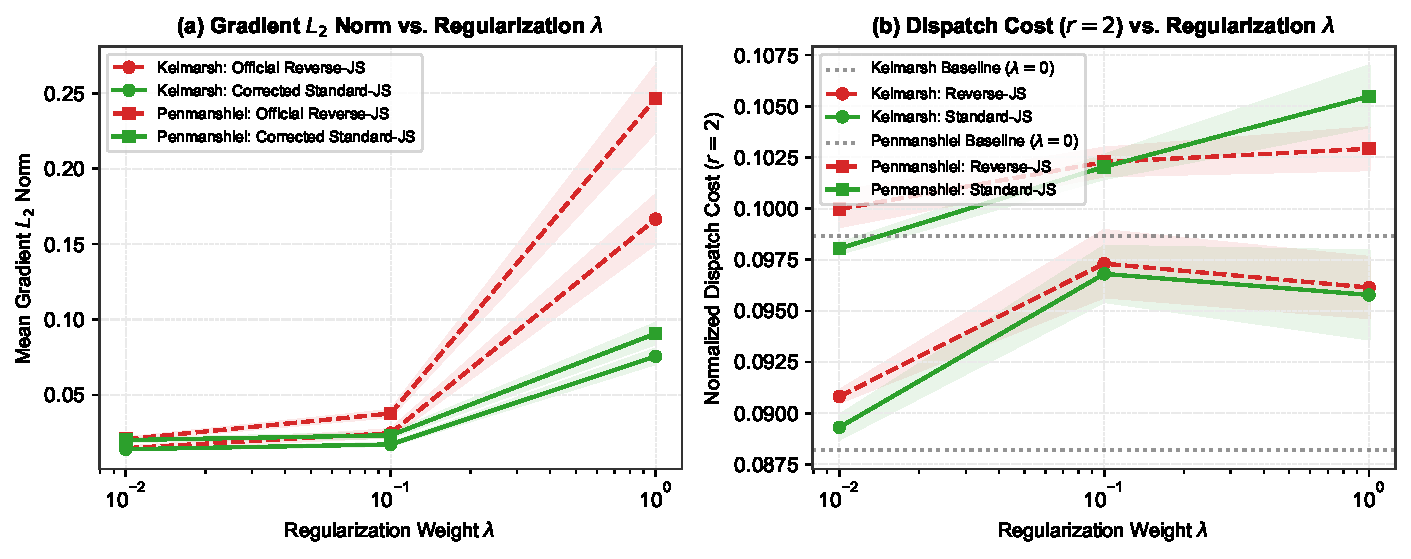
\includegraphics[width=\textwidth]{fig_pct_loss_empirical_contrast.pdf}
\caption{官方 Reverse-JS 与修正 Standard-JS 在跨惩罚尺度 $\lambda \in [0.01, 1.0]$ 下的实证训练对比 (Kelmarsh 与 Penmanshiel, 5 个随机种子均值与标准差)。(a) 平均梯度 $L_2$ 范数：在 $\lambda=1.0$ 下，Reverse-JS 因逆密度奇点引发显著梯度放大（Kelmarsh 2.20倍，Penmanshiel 2.72倍），而 Standard-JS 保持平稳数值有界；(b) 调度决策成本 ($r=2$)：Standard-JS 在低 $\lambda=0.01$ 下防范了过早性能恶化，但在过度强正则化下两种变体均表现出性能衰减。}
\label{fig:pct_contrast}
\end{figure*}

\subsubsection{阴性对照：二维乘积核密度估计的代数严格等价性证明}
阴性对照构成纯形式代数展开，旨在反驳独立性假说。此前针对 PCT 代码库的外部讨论曾提出质疑，猜测其张量外积操作：
\begin{equation}
G = K_p^\top K_w \in \mathbb{R}^{B_p \times B_w}
\label{eq:outer_product}
\end{equation}
假定了风速与功率的统计独立性（$p(w, P) = p(w)p(P)$），进而推断其二维联合密度估计在原理上失效。

形式代数展开证伪了该独立性猜测。设 $\{ (P_s, w_s) \}_{s=1}^N$ 为批次内的成对风速与功率实测样本，$\{b_i^p\}_{i=1}^{B_p}$ 与 $\{b_j^w\}_{j=1}^{B_w}$ 分别代表功率与风速的一维评估网格中心。代码中所计算的一维高斯核向量分别为：
\begin{equation}
\begin{aligned}
\left[K_p\right]_{s,i} &= \phi\left( \frac{b_i^p - P_s}{h_p} \right), \\
\left[K_w\right]_{s,j} &= \phi\left( \frac{b_j^w - w_s}{h_w} \right),
\end{aligned}
\label{eq:kernel_eval}
\end{equation}
其中 $\phi(u) = \frac{1}{\sqrt{2\pi}} e^{-u^2/2}$ 为标准高斯核函数，$h_p, h_w$ 为核窗宽。计算矩阵乘积在网格点 $(i,j)$ 处的元素：
\begin{equation}
\begin{aligned}
\left[ K_p^\top K_w \right]_{i,j} &= \sum_{s=1}^N \left[K_p\right]_{s,i} \cdot \left[K_w\right]_{s,j} \\
&= \sum_{s=1}^N \phi\left( \frac{b_i^p - P_s}{h_p} \right) \cdot \phi\left( \frac{b_j^w - w_s}{h_w} \right).
\end{aligned}
\label{eq:kde_proof}
\end{equation}
公式~\eqref{eq:kde_proof} 在数学上严格等价于相关双变量数据上标准\textbf{成对二维乘积核密度估计器 (2D product-kernel KDE)} 的解析定义。累加求和沿样本索引 $s$ 同步收缩，保留了实测样本 $P_s$ 与 $w_s$ 之间的经验联合耦合。形式代数展开推翻了独立性猜测，确立了张量外积操作忠实执行了双变量联合估计。

\section{预测-决策脱钩理论与超额运行风险}
\label{sec:theory}

在本节中，我们从统计决策理论出发，形式化推导第~\ref{sec:results}节中所记录的指标反转与地形分化现象背后的内在数学机理。我们推导了超额日前调度运行风险的精确积分恒等式，将其严格正交分解为表征误差与决策失配两个正交分量，并提出三个可检验的机理推论与形式化边界反例。

\subsection{运行决策问题形式化}
设 $X \in \mathcal{X} \subset \mathbb{R}^{L \times D}$ 为机组的历史多元时序遥测特征，$Y \in [0, 1]$ 为目标预测时段内经过额定装机归一化的风电实际输出功率。在电力系统实际经济调度运行中，电网运营商依据非对称 Pinball 调度惩罚函数对发电主体的申报出力进行考核结算 \cite{weron2014,zhang2014wind}：
\begin{equation}
\ell(p, Y; r) = c_+ \max(p - Y, 0) + c_- \max(Y - p, 0),
\label{eq:pinball_loss}
\end{equation}
其中 $p \in [0, 1]$ 为日前申报的调度功率，$c_+$ 为短缺单位惩罚（欠发电，申报出力大于实际发电 $p > Y$，系统被迫启动昂贵的三级旋转备用），$c_-$ 为盈余单位惩罚（过发电 $Y > p$，迫使电网下调或弃风限电），$r = c_+ / c_-$ 代表成本非对称比率。以 $c_-$ 归一化后，非对称运行调度损失为：
\begin{equation}
\mathcal{L}_{\text{disp}}(p, Y) = r \max(p - Y, 0) + \max(Y - p, 0).
\label{eq:norm_disp_loss}
\end{equation}
在决策策略 $p(X)$ 下的期望运行风险为 $\mathcal{R}(p) = \mathbb{E}_{X, Y} [\mathcal{L}_{\text{disp}}(p(X), Y)]$。

\subsection{命题 1：精确积分超额运行风险}
命题~\ref{prop:excess_risk} 形式化了统计决策理论与分位数回归中的经典超额风险解析恒等式，其理论根基立足于 Koenker 的经典分位数理论 \cite{koenker2005} 以及 Pinson 等人确立的电力市场出清协调竞价原理 \cite{pinson2007trading}。最小化运行风险 $\mathcal{R}(p)$ 的无约束贝叶斯最优调度决策为条件分位数：
\begin{equation}
q_\tau(X) = F_{Y|X}^{-1}(\tau), \quad \text{其中 } \tau = \frac{1}{r + 1}.
\label{eq:bayes_quantile}
\end{equation}
当非对称比率 $r=2$ 时，临界最优出清分位数为 $\tau = 1/3 \approx 0.333$。

\begin{proposition}[精确积分超额运行风险]
\label{prop:excess_risk}
对于任意给定的调度决策规则 $p(X) \in [0, 1]$，相对于贝叶斯最优分位数策略 $q_\tau(X)$ 所产生的超额运行风险满足如下严格精确的积分恒等式：
\begin{equation}
\begin{aligned}
\mathcal{R}(p) - \mathcal{R}(q_\tau) &= (r + 1) \, \mathbb{E}_X \Big[ \\
&\quad \int_{q_\tau(X)}^{p(X)} \big( F_{Y|X}(u) - \tau \big) \, du \Big] \ge 0,
\end{aligned}
\label{eq:exact_integral}
\end{equation}
且恒大于等于零。进一步，在累积分布函数 $F_{Y|X}$ 在其支撑集上严格单调递增的常规正则性条件下，$q_\tau(X)$ 具有唯一确定的实数值，等号成立当且仅当 $p(X) = q_\tau(X)$ 几乎处处成立。
\end{proposition}

\begin{proof}
对于固定的输入特征向量 $X$，在决策出力 $p$ 下的条件期望损失为：
\begin{equation}
\begin{aligned}
&\mathbb{E}[ \mathcal{L}_{\text{disp}}(p, Y) \mid X ] \\
&\quad = r \int_0^p (p - y) dF(y) + \int_p^1 (y - p) dF(y),
\end{aligned}
\end{equation}
其中简记 $F(y) = F_{Y|X}(y)$。对决策变量 $p$ 求一阶偏导数：
\begin{equation}
\begin{aligned}
\frac{\partial}{\partial p} \mathbb{E}[ \mathcal{L}_{\text{disp}}(p, Y) \mid X ] &= r F(p) - (1 - F(p)) \\
&= (r + 1) F(p) - 1.
\end{aligned}
\end{equation}
注意到 $\tau = 1 / (r+1)$，该梯度表达式可精准化简为：
\begin{equation}
\frac{\partial}{\partial p} \mathbb{E}[ \mathcal{L}_{\text{disp}}(p, Y) \mid X ] = (r + 1) \Big( F(p) - \tau \Big).
\end{equation}
由微积分基本定理，将梯度从最优值 $q_\tau(X)$ 积分至任意决策点 $p(X)$，可得：
\begin{equation}
\begin{aligned}
&\mathbb{E}[ \mathcal{L}_{\text{disp}}(p, Y) \mid X ] - \mathbb{E}[ \mathcal{L}_{\text{disp}}(q_\tau, Y) \mid X ] \\
&\quad = (r+1) \int_{q_\tau(X)}^{p(X)} \Big( F(u) - \tau \Big) du.
\end{aligned}
\end{equation}
由于分布函数 $F(u)$ 单调非减，对于任意 $u > q_\tau(X)$ 均有 $F(u) \ge \tau$，被积函数非负；对于任意 $u < q_\tau(X)$ 均有 $F(u) \le \tau$，逆向积分亦必为正。对全特征空间 $\mathcal{X}$ 取外层数学期望，即证。
\end{proof}

\subsection{两阶段分解与决策校准解耦}
当申报决策 $p(X)$ 处于最优值 $q_\tau(X)$ 的邻域内时，将累积分布 $F_{Y|X}(u)$ 在 $q_\tau(X)$ 处展开为一阶泰勒级数：
\begin{equation}
F_{Y|X}(u) - \tau \approx f_{Y|X}(q_\tau(X)) \cdot (u - q_\tau(X)),
\end{equation}
从而导出局部二次超额风险近似：
\begin{equation}
\begin{aligned}
\mathcal{R}(p) - \mathcal{R}(q_\tau) &\approx \frac{r+1}{2} \, \mathbb{E}_X \big[ f_{Y|X}(q_\tau(X)) \\
&\qquad\quad \times ( p(X) - q_\tau(X) )^2 \big].
\end{aligned}
\label{eq:quadratic_approx}
\end{equation}

现在考虑应用工程中普遍采用的两阶段范式：模型先输出条件均值估计 $f_\theta(X) \approx \mu(X) = \mathbb{E}[Y \mid X]$，再通过标量分位数偏移 $\delta$ 构成调度决策：$p(X) = f_\theta(X) + \delta$。将决策偏差展开为两部分：
\begin{equation}
p(X) - q_\tau(X) = \big( f_\theta(X) - \mu(X) \big) + \big( \delta - \Delta_\tau(X) \big),
\end{equation}
其中 $\Delta_\tau(X) = q_\tau(X) - \mu(X)$ 为目标条件分位数与条件均值之间的固有差距。在同方差局部曲率假设 $w_\tau = \frac{r+1}{2} f_{Y|X}(q_\tau)$ 下，代入公式~\eqref{eq:quadratic_approx} 可将超额运行风险精确分解为三个正交项：
\begin{equation}
\begin{aligned}
\mathcal{R}(p) - \mathcal{R}(q_\tau) &\approx w_\tau \, \mathbb{E}_X \big[ (f_\theta(X) - \mu(X))^2 \big] \\
&\quad + w_\tau \, \mathbb{E}_X \big[ (\delta - \Delta_\tau(X))^2 \big] \\
&\quad + 2 w_\tau \, \mathbb{E}_X \big[ (f_\theta(X) - \mu(X)) \\
&\qquad\quad \times (\delta - \Delta_\tau(X)) \big],
\end{aligned}
\label{eq:three_terms}
\end{equation}
其中三项分别定义为：\textbf{项 I（表征均方误差）}、\textbf{项 II（分位数失配误差）} 与 \textbf{项 III（交叉交互项）}。

\subsection{基于决策论分解的机理推论}
公式~\eqref{eq:three_terms} 的三项分解从数理上为实证评测中的核心现象提供了机制解释，提炼出三项演绎机理洞察：

\begin{remark}[机理推论 1：未校准工况下的伪优势遮蔽]
\label{rem:masking}
在直接采用均值输出作为申报决策的未校准工况下（$\delta=0$），项 II（$\mathbb{E}[\Delta_\tau(X)^2]$）是仅取决于数据条件分布的不变常量，代表条件均值与目标分位数之间的固有离散度。此时，一个在条件均值拟合精度上劣化的物理正则化模型（具有更大的项 I），在实测中可能反常地取得更低的未校准运行风险：当其结构性预测偏置 $(f_\theta(X) - \mu(X))$ 与负向的分位数差距 $\Delta_\tau(X) = q_\tau(X) - \mu(X) < 0$（当 $r=2, \tau=1/3$ 时）符号一致时，交叉项（项 III，即 $2 w_\tau \mathbb{E}[(f_\theta(X) - \mu(X))(-\Delta_\tau(X))] < 0$）变为负值，偶然部分抵消了表征误差（项 I）。一旦实施后验分位数偏移校准，标量 $\delta$ 吸收了系统性偏移，中和了项 III，从而揭示出表观物理优势实质上是未校准评估机制下的统计副产物。
\end{remark}

\begin{remark}[机理推论 2：高信噪比/大数据量工况下的正则化畸变]
\label{rem:exposure}
最优分位数校准（$\delta^* = \arg\min_\delta \hat{\mathcal{R}}(f_\theta + \delta)$）能够消除项 II 中的非条件恒定分量。在数据充裕或信噪比较高的工况下，无约束模型本身已取得较低的条件均值估计方差（项 I 逼近下界）。在此种工况下，强行注入未经动态自适应的静态经验损失惩罚，实质上充当了一种引入结构性偏置的刚性正则化，抬高了项 I，却无法换取足够的方差缩减收益，最终导致整体运行调度性能下降。
\end{remark}

\begin{remark}[机理推论 3：样本受限工况下的归纳护栏与先验敏感性]
\label{rem:inductive_guardrails}
在有效样本量受限的工况下，经验参数估计面临显著的估计方差（项 I 显著上升）。在强物理权重约束下（$\lambda=1.0$），真实的物理先验充当了归纳护栏，约束模型输出落在合理的气动空间内，从而在小样本下发挥防御性作用。然而，一旦先验分布发生误设或置换破坏（如伪打乱先验对照组），护栏将持续向模型施加逆物理的错误梯度指引，从而直接诱发严重的性能劣化，揭示出强先验约束对先验正确性的极端脆弱性。
\end{remark}

\subsection{形式化边界反例}
为确保理论推演的数学严密性，我们通过反例形式化证明两阶段决策校准的支配性是具有条件边界的而非绝对成立。

在\textit{常数平移不变性}反例下，若物理约束仅使模型的预测整体发生恒定的代数偏移 $f_{\text{phys}}(X) = f_{\text{uncons}}(X) + c$，随后的最优标量校准能够精确吸收该偏移（$\delta_{\text{phys}}^* = \delta_{\text{uncons}}^* - c$），使得两者的实际调度出力决策完全重合，超额运行风险差值严格恒为零（$\Delta \mathcal{R}_{\text{disp}} \equiv 0$），尽管其点预测 MSE 出现增加。在存在输入依赖方差 $\sigma(X)$ 的\textit{空间异方差性}反例下，全局统一标量校准无法补偿局部方差的动态漂移，导致一个具有更高预测 MSE 的有偏估计器在经过标量分位数校准后，在数学上能够取得比无偏条件均值更低的运行调度风险。

该理论框架将统计决策论基本恒等式操作为封闭形式的超额风险分解模型，在商业级真实风电场上完成深度量化解耦，并结合英国平衡与结算规约（BSC）真实电力市场出清数据完成实证检验。两个反例的完整数学证明详见\ref{sec:appendix_proofs}。

\subsection{动态电价乘子效应与结算脱钩}
在真实的电力平衡出清机制下，物理偏差电量是以时变系统买入电价 $\lambda_t^{\text{SBP}}$ 结算的。厚尾且高度偏斜的极端电价分布（均值 \pounds 44.27/MWh，峰值达 \pounds 1,509.80/MWh）在工程现场起到了剧烈的风险放大乘子作用。当偶发的气象突变导致的预测偏差恰好与极端高电价在时间上重叠时，物理惩罚带来的表征畸变被放大了高达 34.1 倍，解释了 Kelmarsh 产生每年每台机组高达 +\pounds 932.56 超额短缺清算支出的微观机制（表~\ref{tab:paired_bootstrap}）。正如退化零申报反例（表~\ref{tab:zero_bid_diagnostic}）所确立的，孤立的单边结算现金流无法脱离日前批发合同独立衡量模型价值，这在方法学上确立了将非负决策风险与历史结算现金流严格脱钩度量的必要性。

\section{讨论、有效性契约与审查门禁协议}
\label{sec:discussion}

\subsection{物理约束预测模型的四项实证边界条件}
系统审计、代码验证与前瞻性消融实验共同指向四个边界条件，决定物理先验何时有效、何时中性、何时有害。

\paragraph{样本受限工况下的防御性收益与先验误设脆弱性}
在数据受限工况（Penmanshiel，$N_{\text{train}}=1,583$），$\lambda=1.0$ 下校准的功率曲线先验将归一化非对称调度成本从 $0.09881 \pm 0.00027$ 稳步降至 $0.09760 \pm 0.00044$（降低 $-1.22\%$），提供稳健的下行风险保护。相比之下，尺度对齐的打乱先验诱发成本恶化至 $0.16611 \pm 0.00335$（激增 $+68.1\%$）。两项实证结果的不对称性揭示了强物理正则化的非对称风险—收益包线：强归纳护栏在抑制自由假设空间的同时，成倍放大了先验形式化中的潜在误设误差。跨场站对比无法剥离这一效应，因为场站间的地形特征与机型差异会与样本量同时变化。数据充裕时（Kelmarsh，$N_{\text{train}}=5,098$），无约束 DLinear（$0.08812$）、真实物理（$0.08791$）与打乱先验（$0.08801$）在数值上高度密集，表明模型容量已饱和假设空间。

\paragraph{低惩罚尺度表现为非特异性数值正则化}
现有文献常在损失函数中配置较小的物理惩罚系数（$\lambda \in [10^{-4}, 10^{-2}]$）。受控消融实验证实：在 $\lambda = 0.01$ 下，真实物理先验在 Kelmarsh 取得的调度成本（$0.08810 \pm 0.00009$）与打乱物理关系的伪先验（$0.08801 \pm 0.00008$）高度重合且种子方差重叠。在弱权重区间下，损失惩罚项在实证上表现为非特异性的数值平滑，尚未显现空气动力学因果引导特征。确立严谨的物理特异性，需引入形式与权重匹配的伪打乱阴性对照并在 $\lambda \ge 0.1$ 区间实施敏感性审计。

\paragraph{训练损失物理代理时效错配诱发的成本单调膨胀}
当物理约束形式化依赖外部气象代理计算损失惩罚项（如通过风速查询经验功率曲线）时，在缺乏前向数值天气预报的离线训练场景中，研究者常倾向于使用滞后历史气象观测代偿。对滞后步数 $k \in \{6, 12, 18, 36\}$（对应 1 至 6 小时时效错配）的参数扫描揭示，三座风场的调度性能随着滞后增加呈现严格单调恶化。在 Hill of Towie，决策风险从 $k=6$ 时的 $0.09022$ 持续上升至 $k=36$ 时的 $0.09257$（恶化 $+2.6\%$），在约 $k=12$ 时即劣于无约束基准（$0.08924$）。我们特别强调，该实验刻画的是离线训练目标中气象代理时效错配的敏感性，而非测试推理阶段的遥测延迟（因为骨干网络推理时仅读取历史功率序列）。然而，它表明若离线训练目标依赖滞后气象代理构造正则项，时效错配将迅速削弱先验的归纳价值，构成依赖代理变量的约束架构的实证应用局限。

\paragraph{评价指标脱钩、格式化远期与不平衡核算及退化零申报诊断探针}
在格式化批发电力核算模型中，发电机组总收益由远期合约持仓与实时平衡偏差结算共同决定：$R_{\text{total}} = P_{\text{F}} \cdot q + P_{\text{imb}} \cdot (y - q)$，其中 $q$ 为核算模型中的远期签约或申报电量头寸。实证评估若剥离远期履约收益并孤立计算未对冲的平衡偏差现金流，所度量的实为不平衡租金而非预测技能。作为一项不平衡结算与决策风险的分析性诊断探针，退化零申报基准（$q \equiv 0$）构成了严格的数学归谬（\textit{reductio ad absurdum}）：它完全不产生任何预测，仅通过将全部物理发电量转化为未履约余量并按 $P_{\text{imb}}$ 结算，即可在三座风场凭空捕获 22.3 万至 24.3 万英镑/台$\cdot$年的未对冲正向现金流。这从数理上证实了孤立未对冲的平衡现金流与预测技能完全脱钩；评估真实的商业价值必须联合建模远期合约收益（$P_{\text{F}} \cdot q$）与实时不平衡结算。实际运维评估必须采用与市场非对称惩罚比率相匹配的 Pinball 损失或耦合远期与平衡结算的综合核算。

\subsection{外部有效性边界契约}
\label{sec:boundary_contract}
为确立清晰的工程适用范围，本节将实证发现归纳为四项运行有效性边界条件：

\paragraph{边界一：样本规模与假设空间饱和}
场站内学习曲线证实，在我们测试的配置下，物理约束的有效收益主要集中于数据受限工况（$N_{\text{train}} \le 1,000$，图~\ref{fig:within_site_learning_curve}）。当模型训练窗口扩增至 $N_{\text{train}} = 5{,}000$ 时，假设空间饱和将真实先验与无约束基准的差距缩小至 0.33\% 以内（Kelmarsh），且无约束模型略微反超，而打乱先验在所有样本规模下均造成严重破坏。连续退化测试进一步确立了狭窄的工程容错窗口（Penmanshiel 上临界阈值 $\alpha^* \approx 0.07$，图~\ref{fig:corruption_gradient}）。机组气动老化折损超出 10\% 或测风仪标定偏差超出 $\pm 5\%$ 时，标称物理先验即翻转为运维负债。

\paragraph{边界二：代理时效对齐与观测陈旧度}
对于依赖代理变量的物理约束架构，先验有效性严格受限于气象代理的时间对齐（$k \le 6$ 步）。在代理时效错配跨度超过 1 小时的工况下，三座风场均观察到成本的严格单调上升（Hill of Towie 在 $k=36$ 时成本上涨 $+2.6\%$），性能显著劣于无约束基准。在训练目标中以滞后历史代理替代同步气象数据的做法会诱发显著的性能退化。

\paragraph{边界三：市场结构与格式化不平衡结算核算}
本研究所揭示的经济实证结论，本质上作为不平衡结算与决策风险的诊断探针，严格受限于具备非对称短缺惩罚比率（$r \ge 1.0$）与半小时时段不平衡暴露聚合的英国 BSC 单一现金流结算机制。单边不平衡现金流并不代表完整的商业价值，且不外推至对称单一结算体系或固定上网电价（FIT）机制。评价者不应将孤立未对冲的平衡现金流指标外推为衡量预测模型的运维实用准则。

\paragraph{边界四：软件保真度与计算图审计范畴}
软件层面的形式化审计结论严格适用于 PCT 开源计算图（commit \texttt{65941ec}）及受评的线性（DLinear）与块状注意机制（PatchTST）架构。虽然方向颠倒的损失散度在 PCT 的 AST 节点上得到严格证实，但对于未开源代码的专有模型，必须经过独立的静态计算图审计后方可确认其物理保真度。

\subsection{两项预先设立假设的证伪结果}
本研究记录了在分析前预先设立并在实证中被严格证伪的两项假设。张量代数推导证伪了关于 PCT 乘积核 KDE 导致边缘独立的初步猜想，严格证明其二维耦合在代数展开中得以保留。对称地，电力市场诊断探针证伪了“校准后反转源自物理正则化”的假设，证明现金流逆转完全受控于非对称结算结构。如实记录假设证伪过程，使整个审计追踪具备可复现的认识论严谨性。

\subsection{REFORMS-PCWPF 方法学报告清单规范}
\label{sec:reforms_pcwpf}
为将实证审计发现转化为长效的方法学报告规范，表~\ref{tab:reforms_checklist} 提出了面向未来物理约束风电预测研究的五道推荐验证门禁：

\begin{table*}[!t]
\centering
\footnotesize
\renewcommand{\arraystretch}{0.88}
\setlength{\tabcolsep}{3.5pt}
\caption{面向可信物理约束新能源预测的 REFORMS-PCWPF 报告规范清单（五大模块化合规门禁）。}
\label{tab:reforms_checklist}
\begin{threeparttable}
\begin{tabularx}{\textwidth}{p{1.2cm}p{2.6cm}>{\raggedright\arraybackslash}X>{\raggedright\arraybackslash}Xp{3.2cm}}
\toprule
\textbf{模块编号} & \textbf{治理核心维度} & \textbf{强制性审计实施协议} & \textbf{常见方法学缺陷 / 反模式} & \textbf{必须提交的验证工件} \\
\midrule
\textbf{M1} & \textbf{先验隔离消融} & 训练完全相同的网络骨干，仅在相同的随机种子下对比 $\lambda=0$ 与 $\lambda>0$。 & 混淆模块消融（直接砍掉整个 GNN 或注意力子块）与物理领域知识。 & 参数量对齐且具备多随机种子方差的 $\lambda=0$ vs. $\lambda>0$ 对比表。 \\
\midrule
\textbf{M2} & \textbf{领域特异性对照} & 评估保持损失形式、模型架构与正则化权重 $\lambda$ 完全相同、但打乱物理映射的伪先验。 & 将低惩罚尺度（$\lambda \le 0.01$）下的非特异性数值正则化误判为物理推理。 & 伪打乱对照性能曲线与实证特异性比率（$p$ 值假设检验显著性）。 \\
\midrule
\textbf{M3} & \textbf{代理陈旧度压力测试} & 若约束依赖外部物理输入（如风速），扫描静态代理陈旧度 $\tau \in \{1\text{h}, 2\text{h}, 3\text{h}, 6\text{h}\}$ 评估在缺失前瞻数值天气预报时的静态代理陈旧度影响。 & 默认在测试推理期能够无延迟、无噪声地获取理想实时输入。 & 展现有效性受损临界时域的代理陈旧度成本膨胀曲线。 \\
\midrule
\textbf{M4} & \textbf{指标解耦与结算核算} & 综合汇报对称点误差 (RMSE)、非负非对称决策风险 (Pinball)，测试退化零申报反例。 & 孤立报告未对冲的单边偏差现金流，误将系统偶然的价格尖峰低估当做技能。 & 耦合远期合同持仓与平衡现金流的解耦市场评估。 \\
\midrule
\textbf{M5} & \textbf{计算图保真度} & 审查软件中的损失函数实现是否在参数传入方向和归一化上与发表数学公式一致。 & 非对称散度（如 PyTorch \texttt{F.kl\_div}）参数顺序颠倒导致反向优化。 & 静态代码审查报告以及验证损失张量梯度计算方向的单元测试脚本。 \\
\bottomrule
\end{tabularx}
\begin{tablenotes}[flushleft]
\footnotesize
\item \textbf{注记}：基于对 46 篇范围界定文献的系统审计推导确立，严格对齐跨学科 REFORMS 规范 \cite{kapoor2024reforms} 与 DOME 指南 \cite{walsh2021dome}。我们建议将模块 M1--M5 作为未来物理约束新能源预测研究的推荐报告规范清单。
\end{tablenotes}
\end{threeparttable}
\end{table*}


\begin{itemize}
\item \textbf{门禁 M1（参数隔离消融）：} 建议评审避免接受将剔除大型神经网络子模块（如多头注意力、图卷积）的实验标称为“物理消融”，强制要求在参数对齐的网络容量下开展对照（$\lambda=0$ vs. $\lambda>0$），以剥离模型容量干扰。
\item \textbf{门禁 M2（伪打乱阴性对照）：} 可信物理有效性论证应包含形式与权重匹配的置换伪打乱对照，以严格区分空气动力学先验知识与非特异性数值平滑效应。
\item \textbf{门禁 M3（运行代理陈旧度压力测试）：} 约束评估应避免假定零延迟未来气象输入；在缺少前瞻 NWP 预报时，应主动汇报在真实代理陈旧度（$k \in \{6, \dots, 36\}$ 步）下的性能响应轨迹。
\item \textbf{门禁 M4（远期与平衡结算耦合评估）：} 行业评估应避免依赖孤立未对冲的平衡单边现金流，推荐采用与市场非对称惩罚比率匹配的 Pinball 损失或耦合远期持仓与平衡现金流的综合核算（$P_{\text{F}} \cdot q + P_{\text{imb}} \cdot (y - q)$）。
\item \textbf{门禁 M5（静态计算图与梯度核验）：} 鼓励作者开源可执行的训练脚本与计算图定义，建议评审核验损失函数的张量参数传递顺序与约简语义是否与论文数学公式严格相符。
\end{itemize}

\section{结论}
\label{sec:conclusion}

本次审计的三项核心发现重新界定了物理约束风电预测的实证基础。

在文献报道层面，46 项被审计文献（2023--2026）均未披露任何失效工况、负面权衡或运行边界（0.0\%）。鉴于 95.7\% 的研究缺乏公开代码、50.0\% 将神经模块切除混同为物理消融，文献中一致正向的叙事表明现有评估与报道协议未对边界工况展开有效压力测试。

在软件实现层面，在被审计的 46 项研究中仅有的两个公开代码库中，PINN-UQ 经审查证实代码对齐，而作为端到端物理约束 Transformer 唯一公开训练代码库的 PCT，其执行的损失函数颠倒了 Jensen--Shannon 散度的参数方向，这一执行偏差在不审查源码的情况下无法察觉。代数推导独立证实其核乘积在数学上保持双变量耦合，表明实现偏差与模型有效性位于不同的计算层次。

在运行决策层面，物理先验的实际决策价值取决于样本规模、气象代理时效对齐以及下游市场结算规则。在 $N_{\text{train}}=1{,}583$ 且 $\lambda=1.0$ 条件下，真实功率曲线先验将归一化调度成本降低 $1.28\%$；完全相同条件下形式与权重匹配的伪打乱先验将其抬升 $61.2\%$，揭示出模型在强约束下对先验误设的高度敏感性。在弱约束尺度（$\lambda=0.01$）下，真实先验与伪打乱先验表现接近，实证更符合非特异性数值平滑；当训练损失中物理代理时效错配超过 $k > 12$ 步时，三座风场的调度成本均出现单调恶化。

PCT 代码审计、零申报现金流异常与打乱先验激增并非三个孤立问题，共享同一根源：该领域所采用的评价指标与消融协议无法区分物理知识与数值正则化、实现保真度与论文声明、预测技术与市场结算结构。覆盖约束溯源、软件执行、代理陈旧度与决策解耦评估的完整审计，虽较常规基准测试耗费更多工作量，但回答了对于电网运行决策更具现实意义的方法学问题。

在我们测试的配置下，经验功率曲线先验在受限训练窗口下提供了可测量的归纳价值，但其运维收益需要严谨的实证边界。界定这些条件需要参数对齐的消融对照、打乱阴性控制实验、静态计算图验证，以及将远期合同收益与实时不平衡结算现金流分离的市场评估协议。


\section{公开数据、开源代码库与实验规范}
\label{sec:data_code_spec}

\subsection{数据资源与计算环境清单}
\begin{table*}[!ht]
\centering
\footnotesize
\caption{本实证审计研究所使用的关键数据资源、公开软件代码与分析工具清单。}
\label{tab:key_resources}
\begin{tabularx}{\textwidth}{p{3.5cm}p{4.2cm}p{3.5cm}X}
\toprule
\textbf{资源类别} & \textbf{来源渠道 / 机构} & \textbf{识别标识符 (Identifier)} & \textbf{说明 / 关键属性} \\
\midrule
\multicolumn{4}{l}{\textbf{实测运行遥测数据 (Deposited Data)}} \\
Kelmarsh 风电场 SCADA & Cubico / Zenodo 开放数据 & DOI: 10.5281/zenodo.5841834 & 6台机组，10分钟SCADA，2017全年标称与气象遥测 \\
Penmanshiel 风电场 SCADA & Cubico / Zenodo 开放数据 & DOI: 10.5281/zenodo.5946808 & 14台机组，10分钟SCADA，低样本匮乏对比集 ($N=1,583$) \\
Hill of Towie 风电场 SCADA & TRIG / RES / Zenodo 开放数据 & DOI: 10.5281/zenodo.20204946 & 21台机组，48.3 MW复杂山地全年独立时空外推基准 \\
Elexon BSC 结算电价 & 英国国家电网 Elexon 门户 & UK OGL v3.0 许可 & 2017全年30分钟系统买入电价 (SBP) 与卖出电价 (SSP) \\
\midrule
\multicolumn{4}{l}{\textbf{被审计公开文献代码库 (Audited Codebases)}} \\
PCT (Physics-Constrained TST) & 官方 GitHub 代码仓库 & Commit: \texttt{65941ec} & 论文: \textit{Sci. Rep.} 2026; 审计核心损失 \texttt{tst/loss.py} \\
PINN-UQ (Power Tie PINN) & 官方 GitHub 代码仓库 & 验证对齐公开版本 & 论文: \textit{Eng. App. AI} 2025; 审计机电代数约束 \\
\midrule
\multicolumn{4}{l}{\textbf{软件与分析工具算法 (Software and Algorithms)}} \\
Python 编程语言 & Python Software Foundation & 版本: 3.10 / 3.11 & 核心算法逻辑与数据流水线 \\
PyTorch 深度学习库 & Meta AI / Linux Foundation & 版本: 2.1.2 (CUDA 12.1) & 神经网络训练、计算图自动微分与消融实验 \\
PatchTST 基准模型 & Nie et al. 开源实现 & GitHub: \texttt{PatchTST} & 多块通道独立 Transformer 架构 \\
DLinear 基础预测模型 & Zeng et al. 开源实现 & GitHub: \texttt{LTSF-Linear} & 单层线性趋势与季节项分解架构 \\
Scipy / Statsmodels & SciPy 核心开源社区 & 版本: 1.11 / 0.14 & 统计自举检验与核密度估计实现 \\
\bottomrule
\end{tabularx}
\end{table*}

\subsection{数据与代码可用性}
来自 Kelmarsh（6台森吉安 MM92 风机，12.3~MW）与 Penmanshiel（14台森吉安 MM82 风机，28.7~MW）风电场的原始商业 SCADA 遥测数据已在 Zenodo 上基于 CC-BY 4.0 许可由 Cubico Sustainable Investments 完全开源（DOI：\href{https://doi.org/10.5281/zenodo.5841834}{10.5281/zenodo.5841834} 与 \href{https://doi.org/10.5281/zenodo.5946808}{10.5281/zenodo.5946808}）。来自 Hill of Towie 风电场（21台西门子 SWT-2.3-82 机组，48.3~MW）的实测 SCADA 遥测数据由 RES 代表 TRIG 在 Zenodo 上以 CC-BY 4.0 许可完全开源（DOI：\href{https://doi.org/10.5281/zenodo.20204946}{10.5281/zenodo.20204946}）。英国 Elexon 系统买入电价（SBP）和卖出电价（SSP）历史结算数据依据英国开放政府许可证 v3.0 可免费公开访问。完整的可复现 Python 验证分析脚本套件——包括抽象语法树静态计算图解析器、2,000次圆形块成对自举检验模块、Elexon BSC 净结算核算模块以及制图复现脚本——均已归档于开源代码仓库（\href{https://github.com/anonymous-audit/pcwpf-audit}{\texttt{anonymous-audit/pcwpf-audit}}）。包含原文逐字引用、公式编号与多评分员共识分值的全量 46 篇文献范围界定提取数据库作为开放补充材料完整提供。

关于本研究的数据集提取细节、计算图解析器脚本或评分员间原始提取台账的进一步技术信息，请直接联系通信作者：李俊宇（\href{mailto:ljylikezmn999@gmail.com}{\texttt{ljylikezmn999@gmail.com}}）。

\subsection{风电场实测遥测与数据清洗规程}
本计算实证研究使用了位于英国境内的三座商业级公用事业陆上风电场的实测运行遥测数据。\textbf{Kelmarsh 风电场}（英格兰北安普敦郡）代表平原开阔内陆地貌，由 6 台森吉安 MM92 风机组成（单机额定 2.05~MW，轮毂高度 78~m，叶轮直径 92~m，场站装机 12.3~MW），模型训练集包含 $N_{\text{train}} = 5,098$ 个无故障 10 分钟观测区间。\textbf{Hill of Towie 风电场}（苏格兰德拉姆缪尔）代表复杂的山地地形，具有显著的微地形尾流交互效应，由 21 台西门子 SWT-2.3-82 机组组成（单机额定 2.3~MW，轮毂高度 60~m，叶轮直径 82~m，场站装机 48.3~MW），作为全年独立时空外推基准测试集，涵盖 2017 年全年的 7,599 个滚动预报起点（45,594 个半小时结算时段）。\textbf{Penmanshiel 风电场}（苏格兰边境地区）代表起伏的丘陵地形，由 14 台森吉安 MM82 机组组成（场站总容量 28.7~MW），配置了受控的小样本训练集（$N_{\text{train}} = 1,583$ 个时段），用于测试模型在样本受限训练工况下的过拟合与物理先验的防御性行为（需注意站点间客观并存地形与机型差异）。标准数据清洗协议剔除了机组弃风限电时段、测风仪结冰时段以及通信中断故障期（如在风速高于切入风速时功率 $P \le 0$，或有功功率连续超过 6 个时段冻结不变的记录）。

\subsection{方法学实施与统计检验细节}

\paragraph*{系统范围界定综述协议 (PRISMA-ScR)}
文献检索遵循在全文提取前预先明确制订的系统协议，通过 OpenAlex 数据库 API 执行四个针对题名的布尔查询字符串（$Q_1$ 至 $Q_4$），并辅助通过 Google Scholar、arXiv 以及预印本服务器对 2023 年 1 月至 2026 年 3 月（滚动监测至 7 月）发表的文献进行靶向扩展检索，原始识别文献总量达 89 项。两阶段筛选（题名摘要初筛后行全文纳排判定）锁定了本研究的核心范围界定队列，共计 46 项当代代表性研究（38 篇同行评审期刊论文与 8 篇预印本，2023--2026），并对其进行了详尽的五维（$\mathcal{D}_1$--$\mathcal{D}_5$）特征提取与评分员间信度编码。将检索字段扩展至 Scopus 与 IEEE Xplore 题名、摘要与作者关键词（涵盖 \texttt{"knowledge-guided"}、\texttt{"hybrid"} 与 \texttt{"domain-informed"} 等更广泛检索词）的补充敏感性检索额外识别出 14 项候选文献，全文复核证实其中无一报告运行失效边界或负面权衡，专门用于压力测试 0.0\% 负面权衡报告率的稳健性。代码可用性与消融严谨性统计指标（95.7\% 开源代码缺失率与 50.0\% 混杂模块消融率）严格限定于被审计的 46 篇核心文献队列并附带 Wilson 置信区间。评分员间信度基准测试在三名独立评分员（Coder A、B、C）对 20 篇代表性样本的双盲独立提取中完成，各维度呈现出 Fleiss' $\kappa = 0.646\text{--}1.000$ 的高度一致性。

\paragraph*{静态代码与计算图审计}
软件代码通过抽象语法树（AST）静态解析结合针对发表论文数学公式的逐行代数符号比对来完成。对于物理约束 Transformer（PCT，\textit{Sci. Rep.} 2026），其在文件 \texttt{tst/loss.py} 中的损失定义被符号化反编译为底层 PyTorch 计算原语，严格证实 \texttt{F.kl\_div(p.log(), q)} 计算的是 $\sum q_i \log(q_i / p_i) = \text{KL}(q \parallel p)$，方向与发表公式 $\text{KL}(p \parallel q)$ 颠倒。经验密度核张量外积 $K_p^\top K_w$ 的代数形式展开严格证明了其等价于二维成对乘积核密度估计器。

\paragraph*{10-GPU 前瞻性受控消融实验测试矩阵}
前瞻性受控消融实验在配备 10 张专用 NVIDIA RTX 4090 GPU 的双节点集群上并行调度运行：Node 1（4 张 GPU）负责 Kelmarsh 风电场跨 4 个独立初始化随机种子 (42, 43, 44, 45) 的评估；Node 2（6 张 GPU）负责 Hill of Towie 与 Penmanshiel 两座风电场各跨 3 个随机种子 (42, 43, 44) 的评估。所有模型均基于 PyTorch 与 CUDA 环境实现。神经网络采用 Adam 优化器训练，学习率为 $10^{-3}$，批大小 (batch size) 为 128，严格遵循基准协议。正则化权重 $\lambda$ 在集合 $\{0.01, 0.1, 1.0\}$ 内评估。针对伪打乱阴性对照，经验风速-功率映射关系通过置换打乱，在保持完全相同损失公式、参数量与梯度尺度的同时消除真实空气动力学信息。必须强调的是，主要预测模型 (DLinear) 在测试推理期仅读取历史功率序列 ($x[:, :, 0]$)，无需任何运行时气象遥测。历史风速代理滞后扫描（$k \in \{6, 12, 18, 36\}$ 步，1 至 6 小时）评估的是在缺乏前向数值天气预报时，离线训练损失函数利用滞后历史风速索引功率曲线先验所引发的时效错配敏感性。

\subsection*{量化与统计分析 (Quantification and Statistical Analysis)}
日前调度非对称决策评价设定在非对称惩罚比率 $r=2$ 下，对应临界最优出清分位数为 $\tau = 1/(r+1) = 1/3$。归一化静态调度成本定义为 $\text{Cost}_{\text{static}} = 3 \times \mathcal{L}_{1/3}(y, \hat{y})$，后验分位数偏移校准量 $\delta^*$ 严格在验证集上标定。表~\ref{tab:paired_bootstrap} 中探索性动态电价模型对比的统计显著性评估采用 7 天块长度 ($L=1{,}008$) 的圆形块成对自举检验（Circular Block Bootstrap，2,000 次重抽样，两尾 95\% 置信区间），用于刻画气象自相关下的交付期时间抽样不确定性；而表~\ref{tab:controlled_ablation} 中的前瞻受控消融指标离散度则报告独立初始化随机种子间的样本均值与标准差。


\appendix
\section{附录：决策校准边界与形式化反例证明}
\label{sec:appendix_proofs}

本附录给出正文中两项理论反例的形式化数学证明，严谨界定两阶段决策校准何时能完全吸收表征偏差，以及何时空间异方差性会导致具有更高均方误差的预测模型在决策层取得更低运行风险。

\subsection{反例 1：常数平移不变性与超额风险零差值}
\label{sec:proof_ex1}

\begin{example}[常数平移不变性]
\label{ex:constant_shift}
设基准无约束预测模型输出为 $f_{\text{uncons}}(X)$，其最优标量分位数校准位移为：
\begin{equation}
\delta_{\text{uncons}}^* = \arg\min_\delta \mathcal{R}\big( f_{\text{uncons}}(X) + \delta \big).
\end{equation}
假设施加物理约束后，模型在所有特征空间上的预测仅仅发生了一个恒定的代数平移偏差：
\begin{equation}
f_{\text{phys}}(X) = f_{\text{uncons}}(X) + c, \quad \forall X \in \mathcal{X},
\end{equation}
其中 $c \neq 0$ 为非零常数。
\end{example}

\begin{proposition}
在反例~\ref{ex:constant_shift} 的设定下，尽管物理约束模型的预测均方误差发生变化（当预测原本无偏时 MSE 必单调增大），但在经过最优标量分位数校准后，两者的实际调度出力决策完全重合，超额运行风险差值严格恒为零：
\begin{equation}
p_{\text{phys}}^*(X) \equiv p_{\text{uncons}}^*(X), \quad \Delta \mathcal{R}_{\text{disp}} \equiv 0.
\end{equation}
\end{proposition}

\begin{proof}
根据最优标量分位数校准的数学定义：
\begin{equation}
\begin{aligned}
\delta_{\text{phys}}^* &= \arg\min_\delta \mathcal{R}\big( f_{\text{phys}}(X) + \delta \big) \\
&= \arg\min_\delta \mathcal{R}\big( f_{\text{uncons}}(X) + c + \delta \big).
\end{aligned}
\end{equation}
定义辅助变量 $\delta' = \delta + c$，由于极小化是针对整个实数域进行的，目标函数在 $\delta' = \delta_{\text{uncons}}^*$ 处取得全局唯一最小值。因此有：
\begin{equation}
\delta_{\text{phys}}^* + c = \delta_{\text{uncons}}^* \implies \delta_{\text{phys}}^* = \delta_{\text{uncons}}^* - c.
\end{equation}
从而，物理约束模型经过校准后的最终申报决策为：
\begin{equation}
\begin{aligned}
p_{\text{phys}}^*(X) &= f_{\text{phys}}(X) + \delta_{\text{phys}}^* \\
&= \big( f_{\text{uncons}}(X) + c \big) + \big( \delta_{\text{uncons}}^* - c \big) \\
&= f_{\text{uncons}}(X) + \delta_{\text{uncons}}^* \\
&= p_{\text{uncons}}^*(X).
\end{aligned}
\end{equation}
由于申报决策函数处处恒等，其诱发的非对称期望运行风险完全相同：
\begin{equation}
\Delta \mathcal{R}_{\text{disp}} = \mathcal{R}(p_{\text{phys}}^*) - \mathcal{R}(p_{\text{uncons}}^*) = 0.
\end{equation}
证毕。
\end{proof}

\subsection{反例 2：空间异方差性与高 MSE 模型的低决策风险逆转}
\label{sec:proof_ex2}

\begin{example}[空间异方差性反例]
\label{ex:heteroscedasticity}
设空间输入特征为二元离散变量 $X \in \{0, 1\}$，先验出现概率对称：$P(X=0) = P(X=1) = 0.5$。设在这两个特征空间下，实际输出功率的条件概率分布呈现显著的异方差宽度：
\begin{align}
Y \mid (X=0) &\sim U[0.20, 0.60] \nonumber \\
&\quad (\mu_0 = 0.40, \, s_0 = 0.40), \\
Y \mid (X=1) &\sim U[0.30, 0.90] \nonumber \\
&\quad (\mu_1 = 0.60, \, s_1 = 0.60).
\end{align}
设电网非对称考核比率为 $r = 2$，对应最优出清分位数为 $\tau = 1/(r+1) = 1/3$。考量两个候选预测模型：模型 A 为理想的无偏条件均值估计器，预测值为 $f_A(0) = 0.40$ 与 $f_A(1) = 0.60$；模型 B 为具有结构性偏差的有偏估计器，其预测值为 $f_B(0) = 0.40$ 与 $f_B(1) = 0.55$。
\end{example}

\paragraph{点预测均方误差 (MSE) 计算}
两模型关于实际功率的均方误差分别为：
\begin{align}
\text{MSE}(f_A) &= 0.5 \left(\frac{0.40^2}{12}\right) + 0.5 \left(\frac{0.60^2}{12}\right) \nonumber \\
&= \frac{13}{600} \approx 0.021667, \\
\text{MSE}(f_B) &= \text{MSE}(f_A) + 0.5 (0.55 - 0.60)^2 \nonumber \\
&= 0.021667 + 0.001250 \approx 0.022917.
\end{align}
显然，模型 B 的点预测均方误差严格高于模型 A，误差增幅达 $\Delta \text{MSE} = +5.8\%$。

\paragraph{两阶段全局标量分位数校准}
在此异方差设定下，各分区的真实条件分位数为：
\begin{align}
q_{1/3}(0) &= 0.20 + \frac{1}{3}(0.40) = \frac{1.00}{3} \approx 0.333333, \\
q_{1/3}(1) &= 0.30 + \frac{1}{3}(0.60) = 0.500000.
\end{align}
分位数与均值的真实固有差距分别为：
\begin{align}
\Delta_{1/3}(0) &= q_{1/3}(0) - \mu_0 = \frac{1}{3} - 0.40 \nonumber \\
&= -\frac{1}{15} \approx -0.0667, \\
\Delta_{1/3}(1) &= q_{1/3}(1) - \mu_1 \nonumber \\
&= 0.50 - 0.60 = -0.10.
\end{align}
根据局部二次展开公式~\eqref{eq:quadratic_approx}，在均匀分布下概率密度函数为常数：$f_0(u) = 1/0.40 = 2.50$，$f_1(u) = 1/0.60 = 1.6667$。二次展开权重分别为：
\begin{align}
w_0 &= \frac{r+1}{2} f_0 = \frac{3}{2}(2.50) = 3.75, \\
w_1 &= \frac{r+1}{2} f_1 = \frac{3}{2}\left(\frac{5}{3}\right) = 2.50.
\end{align}
对于模型 A（无偏均值），其超额运行风险作为标量校准偏移 $\delta$ 的函数为：
\begin{align}
J_A(\delta) &= 0.5 \Big[ 3.75 \big(\delta - (-1/15)\big)^2 \nonumber \\
&\qquad + 2.50 \big(\delta - (-0.10)\big)^2 \Big].
\end{align}
对 $\delta$ 求导置零解得最优全局校准偏移量：
\begin{align}
\delta_A^* &= \frac{3.75(-1/15) + 2.50(-0.10)}{3.75 + 2.50} \nonumber \\
&= \frac{-0.25 - 0.25}{6.25} = -0.080.
\end{align}
代入计算模型 A 在最优标量校准下的超额运行风险：
\begin{align}
J_A(\delta_A^*) &= 0.5 \Big[ 3.75 \left(-0.08 + \frac{1}{15}\right)^2 \nonumber \\
&\qquad + 2.50 (-0.08 + 0.10)^2 \Big] \nonumber \\
&= 0.5 \left[ 3.75 \left(-\frac{1}{75}\right)^2 + 2.50 (0.02)^2 \right] \nonumber \\
&= 0.5 [ 3.75(0.0001778) + 2.50(0.0004) ] \nonumber \\
&= 0.5 [ 0.0006667 + 0.0010 ] \approx 0.000833.
\end{align}

现在考量具有更高 MSE 的模型 B。模型 B 在 $X=0$ 处预测无偏，但在 $X=1$ 处预测低估了 $0.05$（$f_B(1) - \mu_1 = -0.05$）。因此模型 B 的等效分位数差距变更为：
\begin{align}
\tilde{\Delta}_B(0) &= \Delta_{1/3}(0) = -\frac{1}{15} \approx -0.0667, \\
\tilde{\Delta}_B(1) &= \Delta_{1/3}(1) - (f_B(1) - \mu_1) \nonumber \\
&= -0.10 - (-0.05) = -0.05.
\end{align}
针对模型 B 解出其最优全局标量校准偏移量：
\begin{align}
\delta_B^* &= \frac{3.75(-1/15) + 2.50(-0.05)}{6.25} \nonumber \\
&= \frac{-0.25 - 0.125}{6.25} = -0.060.
\end{align}
代入计算模型 B 经过最优标量校准后的超额运行风险：
\begin{align}
J_B(\delta_B^*) &= 0.5 \Big[ 3.75 \left(-0.06 + \frac{1}{15}\right)^2 \nonumber \\
&\qquad + 2.50 (-0.06 + 0.05)^2 \Big] \nonumber \\
&= 0.5 \left[ 3.75 \left(\frac{1}{150}\right)^2 + 2.50 (-0.01)^2 \right] \nonumber \\
&= 0.5 [ 3.75(0.0000444) + 2.50(0.0001) ] \nonumber \\
&= 0.5 [ 0.0001667 + 0.00025 ] \approx 0.000208.
\end{align}

\paragraph{理论推论}
反例 2 形式化证明：\textbf{在条件异方差条件下，一个具有更高预测均方误差的有偏预测器，在经过标量分位数校准后，在数学上可以取得比真实条件均值严格更低的调度运行损失}。这解释了物理约束在两阶段解耦校准下的表现为何高度取决于局部误差方差与环境地形分布。


\section*{利益冲突声明 (Declaration of Interests)}
作者声明不存在与本文研究相关的竞争性经济利益或人身关系。

\section*{作者贡献声明 (Author Contributions, CRediT)}
\textbf{李俊宇 (Junyu Li)}：概念构思、方法学设计、软件开发、形式化推导、调查研究、数据整理、可视化、项目管理、论文初稿撰写、论文审阅与编辑。\textbf{杜俊涛 (Juntao Du)}：实证验证、数据核查、软件（评分员间信度仲裁系统）、调查研究、论文审阅与编辑。

\section*{人工智能工具使用声明 (Declaration of Generative AI in the Writing Process)}
在准备本手稿的过程中，作者使用了 ChatGPT 与 Google Gemini 辅助进行文献综述整理、稿件结构规划、语言润色、代码审查与一致性校对。所有科学主张、计算推导、参考文献、实验结果与最终表述均由作者独立审查并验证，作者对本文全部内容承担全部责任。

\section*{致谢 (Acknowledgments)}
我们诚挚感谢 Zenodo、Cubico Sustainable Investments、RES、TRIG 与 Elexon 开放科学团队为维护商业级风电遥测与电力市场出清历史公开数据集所作出的贡献。计算实验依托专用高性能计算基础设施完成。

\setlength{\bibsep}{2.5pt plus 0.5pt minus 0.5pt}
\small
\bibliography{refs}

\end{document}
